
% Default to the notebook output style

    


% Inherit from the specified cell style.




    
\documentclass[11pt]{article}

    
    
    \usepackage[T1]{fontenc}
    % Nicer default font (+ math font) than Computer Modern for most use cases
    \usepackage{mathpazo}

    % Basic figure setup, for now with no caption control since it's done
    % automatically by Pandoc (which extracts ![](path) syntax from Markdown).
    \usepackage{graphicx}
    % We will generate all images so they have a width \maxwidth. This means
    % that they will get their normal width if they fit onto the page, but
    % are scaled down if they would overflow the margins.
    \makeatletter
    \def\maxwidth{\ifdim\Gin@nat@width>\linewidth\linewidth
    \else\Gin@nat@width\fi}
    \makeatother
    \let\Oldincludegraphics\includegraphics
    % Set max figure width to be 80% of text width, for now hardcoded.
    \renewcommand{\includegraphics}[1]{\Oldincludegraphics[width=.8\maxwidth]{#1}}
    % Ensure that by default, figures have no caption (until we provide a
    % proper Figure object with a Caption API and a way to capture that
    % in the conversion process - todo).
    \usepackage{caption}
    \DeclareCaptionLabelFormat{nolabel}{}
    \captionsetup{labelformat=nolabel}

    \usepackage{adjustbox} % Used to constrain images to a maximum size 
    \usepackage{xcolor} % Allow colors to be defined
    \usepackage{enumerate} % Needed for markdown enumerations to work
    \usepackage{geometry} % Used to adjust the document margins
    \usepackage{amsmath} % Equations
    \usepackage{amssymb} % Equations
    \usepackage{textcomp} % defines textquotesingle
    % Hack from http://tex.stackexchange.com/a/47451/13684:
    \AtBeginDocument{%
        \def\PYZsq{\textquotesingle}% Upright quotes in Pygmentized code
    }
    \usepackage{upquote} % Upright quotes for verbatim code
    \usepackage{eurosym} % defines \euro
    \usepackage[mathletters]{ucs} % Extended unicode (utf-8) support
    \usepackage[utf8x]{inputenc} % Allow utf-8 characters in the tex document
    \usepackage{fancyvrb} % verbatim replacement that allows latex
    \usepackage{grffile} % extends the file name processing of package graphics 
                         % to support a larger range 
    % The hyperref package gives us a pdf with properly built
    % internal navigation ('pdf bookmarks' for the table of contents,
    % internal cross-reference links, web links for URLs, etc.)
    \usepackage{hyperref}
    \usepackage{longtable} % longtable support required by pandoc >1.10
    \usepackage{booktabs}  % table support for pandoc > 1.12.2
    \usepackage[inline]{enumitem} % IRkernel/repr support (it uses the enumerate* environment)
    \usepackage[normalem]{ulem} % ulem is needed to support strikethroughs (\sout)
                                % normalem makes italics be italics, not underlines
    

    
    
    % Colors for the hyperref package
    \definecolor{urlcolor}{rgb}{0,.145,.698}
    \definecolor{linkcolor}{rgb}{.71,0.21,0.01}
    \definecolor{citecolor}{rgb}{.12,.54,.11}

    % ANSI colors
    \definecolor{ansi-black}{HTML}{3E424D}
    \definecolor{ansi-black-intense}{HTML}{282C36}
    \definecolor{ansi-red}{HTML}{E75C58}
    \definecolor{ansi-red-intense}{HTML}{B22B31}
    \definecolor{ansi-green}{HTML}{00A250}
    \definecolor{ansi-green-intense}{HTML}{007427}
    \definecolor{ansi-yellow}{HTML}{DDB62B}
    \definecolor{ansi-yellow-intense}{HTML}{B27D12}
    \definecolor{ansi-blue}{HTML}{208FFB}
    \definecolor{ansi-blue-intense}{HTML}{0065CA}
    \definecolor{ansi-magenta}{HTML}{D160C4}
    \definecolor{ansi-magenta-intense}{HTML}{A03196}
    \definecolor{ansi-cyan}{HTML}{60C6C8}
    \definecolor{ansi-cyan-intense}{HTML}{258F8F}
    \definecolor{ansi-white}{HTML}{C5C1B4}
    \definecolor{ansi-white-intense}{HTML}{A1A6B2}

    % commands and environments needed by pandoc snippets
    % extracted from the output of `pandoc -s`
    \providecommand{\tightlist}{%
      \setlength{\itemsep}{0pt}\setlength{\parskip}{0pt}}
    \DefineVerbatimEnvironment{Highlighting}{Verbatim}{commandchars=\\\{\}}
    % Add ',fontsize=\small' for more characters per line
    \newenvironment{Shaded}{}{}
    \newcommand{\KeywordTok}[1]{\textcolor[rgb]{0.00,0.44,0.13}{\textbf{{#1}}}}
    \newcommand{\DataTypeTok}[1]{\textcolor[rgb]{0.56,0.13,0.00}{{#1}}}
    \newcommand{\DecValTok}[1]{\textcolor[rgb]{0.25,0.63,0.44}{{#1}}}
    \newcommand{\BaseNTok}[1]{\textcolor[rgb]{0.25,0.63,0.44}{{#1}}}
    \newcommand{\FloatTok}[1]{\textcolor[rgb]{0.25,0.63,0.44}{{#1}}}
    \newcommand{\CharTok}[1]{\textcolor[rgb]{0.25,0.44,0.63}{{#1}}}
    \newcommand{\StringTok}[1]{\textcolor[rgb]{0.25,0.44,0.63}{{#1}}}
    \newcommand{\CommentTok}[1]{\textcolor[rgb]{0.38,0.63,0.69}{\textit{{#1}}}}
    \newcommand{\OtherTok}[1]{\textcolor[rgb]{0.00,0.44,0.13}{{#1}}}
    \newcommand{\AlertTok}[1]{\textcolor[rgb]{1.00,0.00,0.00}{\textbf{{#1}}}}
    \newcommand{\FunctionTok}[1]{\textcolor[rgb]{0.02,0.16,0.49}{{#1}}}
    \newcommand{\RegionMarkerTok}[1]{{#1}}
    \newcommand{\ErrorTok}[1]{\textcolor[rgb]{1.00,0.00,0.00}{\textbf{{#1}}}}
    \newcommand{\NormalTok}[1]{{#1}}
    
    % Additional commands for more recent versions of Pandoc
    \newcommand{\ConstantTok}[1]{\textcolor[rgb]{0.53,0.00,0.00}{{#1}}}
    \newcommand{\SpecialCharTok}[1]{\textcolor[rgb]{0.25,0.44,0.63}{{#1}}}
    \newcommand{\VerbatimStringTok}[1]{\textcolor[rgb]{0.25,0.44,0.63}{{#1}}}
    \newcommand{\SpecialStringTok}[1]{\textcolor[rgb]{0.73,0.40,0.53}{{#1}}}
    \newcommand{\ImportTok}[1]{{#1}}
    \newcommand{\DocumentationTok}[1]{\textcolor[rgb]{0.73,0.13,0.13}{\textit{{#1}}}}
    \newcommand{\AnnotationTok}[1]{\textcolor[rgb]{0.38,0.63,0.69}{\textbf{\textit{{#1}}}}}
    \newcommand{\CommentVarTok}[1]{\textcolor[rgb]{0.38,0.63,0.69}{\textbf{\textit{{#1}}}}}
    \newcommand{\VariableTok}[1]{\textcolor[rgb]{0.10,0.09,0.49}{{#1}}}
    \newcommand{\ControlFlowTok}[1]{\textcolor[rgb]{0.00,0.44,0.13}{\textbf{{#1}}}}
    \newcommand{\OperatorTok}[1]{\textcolor[rgb]{0.40,0.40,0.40}{{#1}}}
    \newcommand{\BuiltInTok}[1]{{#1}}
    \newcommand{\ExtensionTok}[1]{{#1}}
    \newcommand{\PreprocessorTok}[1]{\textcolor[rgb]{0.74,0.48,0.00}{{#1}}}
    \newcommand{\AttributeTok}[1]{\textcolor[rgb]{0.49,0.56,0.16}{{#1}}}
    \newcommand{\InformationTok}[1]{\textcolor[rgb]{0.38,0.63,0.69}{\textbf{\textit{{#1}}}}}
    \newcommand{\WarningTok}[1]{\textcolor[rgb]{0.38,0.63,0.69}{\textbf{\textit{{#1}}}}}
    
    
    % Define a nice break command that doesn't care if a line doesn't already
    % exist.
    \def\br{\hspace*{\fill} \\* }
    % Math Jax compatability definitions
    \def\gt{>}
    \def\lt{<}
    % Document parameters
    \title{Laboratorio-4}
    
    
    

    % Pygments definitions
    
\makeatletter
\def\PY@reset{\let\PY@it=\relax \let\PY@bf=\relax%
    \let\PY@ul=\relax \let\PY@tc=\relax%
    \let\PY@bc=\relax \let\PY@ff=\relax}
\def\PY@tok#1{\csname PY@tok@#1\endcsname}
\def\PY@toks#1+{\ifx\relax#1\empty\else%
    \PY@tok{#1}\expandafter\PY@toks\fi}
\def\PY@do#1{\PY@bc{\PY@tc{\PY@ul{%
    \PY@it{\PY@bf{\PY@ff{#1}}}}}}}
\def\PY#1#2{\PY@reset\PY@toks#1+\relax+\PY@do{#2}}

\expandafter\def\csname PY@tok@w\endcsname{\def\PY@tc##1{\textcolor[rgb]{0.73,0.73,0.73}{##1}}}
\expandafter\def\csname PY@tok@c\endcsname{\let\PY@it=\textit\def\PY@tc##1{\textcolor[rgb]{0.25,0.50,0.50}{##1}}}
\expandafter\def\csname PY@tok@cp\endcsname{\def\PY@tc##1{\textcolor[rgb]{0.74,0.48,0.00}{##1}}}
\expandafter\def\csname PY@tok@k\endcsname{\let\PY@bf=\textbf\def\PY@tc##1{\textcolor[rgb]{0.00,0.50,0.00}{##1}}}
\expandafter\def\csname PY@tok@kp\endcsname{\def\PY@tc##1{\textcolor[rgb]{0.00,0.50,0.00}{##1}}}
\expandafter\def\csname PY@tok@kt\endcsname{\def\PY@tc##1{\textcolor[rgb]{0.69,0.00,0.25}{##1}}}
\expandafter\def\csname PY@tok@o\endcsname{\def\PY@tc##1{\textcolor[rgb]{0.40,0.40,0.40}{##1}}}
\expandafter\def\csname PY@tok@ow\endcsname{\let\PY@bf=\textbf\def\PY@tc##1{\textcolor[rgb]{0.67,0.13,1.00}{##1}}}
\expandafter\def\csname PY@tok@nb\endcsname{\def\PY@tc##1{\textcolor[rgb]{0.00,0.50,0.00}{##1}}}
\expandafter\def\csname PY@tok@nf\endcsname{\def\PY@tc##1{\textcolor[rgb]{0.00,0.00,1.00}{##1}}}
\expandafter\def\csname PY@tok@nc\endcsname{\let\PY@bf=\textbf\def\PY@tc##1{\textcolor[rgb]{0.00,0.00,1.00}{##1}}}
\expandafter\def\csname PY@tok@nn\endcsname{\let\PY@bf=\textbf\def\PY@tc##1{\textcolor[rgb]{0.00,0.00,1.00}{##1}}}
\expandafter\def\csname PY@tok@ne\endcsname{\let\PY@bf=\textbf\def\PY@tc##1{\textcolor[rgb]{0.82,0.25,0.23}{##1}}}
\expandafter\def\csname PY@tok@nv\endcsname{\def\PY@tc##1{\textcolor[rgb]{0.10,0.09,0.49}{##1}}}
\expandafter\def\csname PY@tok@no\endcsname{\def\PY@tc##1{\textcolor[rgb]{0.53,0.00,0.00}{##1}}}
\expandafter\def\csname PY@tok@nl\endcsname{\def\PY@tc##1{\textcolor[rgb]{0.63,0.63,0.00}{##1}}}
\expandafter\def\csname PY@tok@ni\endcsname{\let\PY@bf=\textbf\def\PY@tc##1{\textcolor[rgb]{0.60,0.60,0.60}{##1}}}
\expandafter\def\csname PY@tok@na\endcsname{\def\PY@tc##1{\textcolor[rgb]{0.49,0.56,0.16}{##1}}}
\expandafter\def\csname PY@tok@nt\endcsname{\let\PY@bf=\textbf\def\PY@tc##1{\textcolor[rgb]{0.00,0.50,0.00}{##1}}}
\expandafter\def\csname PY@tok@nd\endcsname{\def\PY@tc##1{\textcolor[rgb]{0.67,0.13,1.00}{##1}}}
\expandafter\def\csname PY@tok@s\endcsname{\def\PY@tc##1{\textcolor[rgb]{0.73,0.13,0.13}{##1}}}
\expandafter\def\csname PY@tok@sd\endcsname{\let\PY@it=\textit\def\PY@tc##1{\textcolor[rgb]{0.73,0.13,0.13}{##1}}}
\expandafter\def\csname PY@tok@si\endcsname{\let\PY@bf=\textbf\def\PY@tc##1{\textcolor[rgb]{0.73,0.40,0.53}{##1}}}
\expandafter\def\csname PY@tok@se\endcsname{\let\PY@bf=\textbf\def\PY@tc##1{\textcolor[rgb]{0.73,0.40,0.13}{##1}}}
\expandafter\def\csname PY@tok@sr\endcsname{\def\PY@tc##1{\textcolor[rgb]{0.73,0.40,0.53}{##1}}}
\expandafter\def\csname PY@tok@ss\endcsname{\def\PY@tc##1{\textcolor[rgb]{0.10,0.09,0.49}{##1}}}
\expandafter\def\csname PY@tok@sx\endcsname{\def\PY@tc##1{\textcolor[rgb]{0.00,0.50,0.00}{##1}}}
\expandafter\def\csname PY@tok@m\endcsname{\def\PY@tc##1{\textcolor[rgb]{0.40,0.40,0.40}{##1}}}
\expandafter\def\csname PY@tok@gh\endcsname{\let\PY@bf=\textbf\def\PY@tc##1{\textcolor[rgb]{0.00,0.00,0.50}{##1}}}
\expandafter\def\csname PY@tok@gu\endcsname{\let\PY@bf=\textbf\def\PY@tc##1{\textcolor[rgb]{0.50,0.00,0.50}{##1}}}
\expandafter\def\csname PY@tok@gd\endcsname{\def\PY@tc##1{\textcolor[rgb]{0.63,0.00,0.00}{##1}}}
\expandafter\def\csname PY@tok@gi\endcsname{\def\PY@tc##1{\textcolor[rgb]{0.00,0.63,0.00}{##1}}}
\expandafter\def\csname PY@tok@gr\endcsname{\def\PY@tc##1{\textcolor[rgb]{1.00,0.00,0.00}{##1}}}
\expandafter\def\csname PY@tok@ge\endcsname{\let\PY@it=\textit}
\expandafter\def\csname PY@tok@gs\endcsname{\let\PY@bf=\textbf}
\expandafter\def\csname PY@tok@gp\endcsname{\let\PY@bf=\textbf\def\PY@tc##1{\textcolor[rgb]{0.00,0.00,0.50}{##1}}}
\expandafter\def\csname PY@tok@go\endcsname{\def\PY@tc##1{\textcolor[rgb]{0.53,0.53,0.53}{##1}}}
\expandafter\def\csname PY@tok@gt\endcsname{\def\PY@tc##1{\textcolor[rgb]{0.00,0.27,0.87}{##1}}}
\expandafter\def\csname PY@tok@err\endcsname{\def\PY@bc##1{\setlength{\fboxsep}{0pt}\fcolorbox[rgb]{1.00,0.00,0.00}{1,1,1}{\strut ##1}}}
\expandafter\def\csname PY@tok@kc\endcsname{\let\PY@bf=\textbf\def\PY@tc##1{\textcolor[rgb]{0.00,0.50,0.00}{##1}}}
\expandafter\def\csname PY@tok@kd\endcsname{\let\PY@bf=\textbf\def\PY@tc##1{\textcolor[rgb]{0.00,0.50,0.00}{##1}}}
\expandafter\def\csname PY@tok@kn\endcsname{\let\PY@bf=\textbf\def\PY@tc##1{\textcolor[rgb]{0.00,0.50,0.00}{##1}}}
\expandafter\def\csname PY@tok@kr\endcsname{\let\PY@bf=\textbf\def\PY@tc##1{\textcolor[rgb]{0.00,0.50,0.00}{##1}}}
\expandafter\def\csname PY@tok@bp\endcsname{\def\PY@tc##1{\textcolor[rgb]{0.00,0.50,0.00}{##1}}}
\expandafter\def\csname PY@tok@fm\endcsname{\def\PY@tc##1{\textcolor[rgb]{0.00,0.00,1.00}{##1}}}
\expandafter\def\csname PY@tok@vc\endcsname{\def\PY@tc##1{\textcolor[rgb]{0.10,0.09,0.49}{##1}}}
\expandafter\def\csname PY@tok@vg\endcsname{\def\PY@tc##1{\textcolor[rgb]{0.10,0.09,0.49}{##1}}}
\expandafter\def\csname PY@tok@vi\endcsname{\def\PY@tc##1{\textcolor[rgb]{0.10,0.09,0.49}{##1}}}
\expandafter\def\csname PY@tok@vm\endcsname{\def\PY@tc##1{\textcolor[rgb]{0.10,0.09,0.49}{##1}}}
\expandafter\def\csname PY@tok@sa\endcsname{\def\PY@tc##1{\textcolor[rgb]{0.73,0.13,0.13}{##1}}}
\expandafter\def\csname PY@tok@sb\endcsname{\def\PY@tc##1{\textcolor[rgb]{0.73,0.13,0.13}{##1}}}
\expandafter\def\csname PY@tok@sc\endcsname{\def\PY@tc##1{\textcolor[rgb]{0.73,0.13,0.13}{##1}}}
\expandafter\def\csname PY@tok@dl\endcsname{\def\PY@tc##1{\textcolor[rgb]{0.73,0.13,0.13}{##1}}}
\expandafter\def\csname PY@tok@s2\endcsname{\def\PY@tc##1{\textcolor[rgb]{0.73,0.13,0.13}{##1}}}
\expandafter\def\csname PY@tok@sh\endcsname{\def\PY@tc##1{\textcolor[rgb]{0.73,0.13,0.13}{##1}}}
\expandafter\def\csname PY@tok@s1\endcsname{\def\PY@tc##1{\textcolor[rgb]{0.73,0.13,0.13}{##1}}}
\expandafter\def\csname PY@tok@mb\endcsname{\def\PY@tc##1{\textcolor[rgb]{0.40,0.40,0.40}{##1}}}
\expandafter\def\csname PY@tok@mf\endcsname{\def\PY@tc##1{\textcolor[rgb]{0.40,0.40,0.40}{##1}}}
\expandafter\def\csname PY@tok@mh\endcsname{\def\PY@tc##1{\textcolor[rgb]{0.40,0.40,0.40}{##1}}}
\expandafter\def\csname PY@tok@mi\endcsname{\def\PY@tc##1{\textcolor[rgb]{0.40,0.40,0.40}{##1}}}
\expandafter\def\csname PY@tok@il\endcsname{\def\PY@tc##1{\textcolor[rgb]{0.40,0.40,0.40}{##1}}}
\expandafter\def\csname PY@tok@mo\endcsname{\def\PY@tc##1{\textcolor[rgb]{0.40,0.40,0.40}{##1}}}
\expandafter\def\csname PY@tok@ch\endcsname{\let\PY@it=\textit\def\PY@tc##1{\textcolor[rgb]{0.25,0.50,0.50}{##1}}}
\expandafter\def\csname PY@tok@cm\endcsname{\let\PY@it=\textit\def\PY@tc##1{\textcolor[rgb]{0.25,0.50,0.50}{##1}}}
\expandafter\def\csname PY@tok@cpf\endcsname{\let\PY@it=\textit\def\PY@tc##1{\textcolor[rgb]{0.25,0.50,0.50}{##1}}}
\expandafter\def\csname PY@tok@c1\endcsname{\let\PY@it=\textit\def\PY@tc##1{\textcolor[rgb]{0.25,0.50,0.50}{##1}}}
\expandafter\def\csname PY@tok@cs\endcsname{\let\PY@it=\textit\def\PY@tc##1{\textcolor[rgb]{0.25,0.50,0.50}{##1}}}

\def\PYZbs{\char`\\}
\def\PYZus{\char`\_}
\def\PYZob{\char`\{}
\def\PYZcb{\char`\}}
\def\PYZca{\char`\^}
\def\PYZam{\char`\&}
\def\PYZlt{\char`\<}
\def\PYZgt{\char`\>}
\def\PYZsh{\char`\#}
\def\PYZpc{\char`\%}
\def\PYZdl{\char`\$}
\def\PYZhy{\char`\-}
\def\PYZsq{\char`\'}
\def\PYZdq{\char`\"}
\def\PYZti{\char`\~}
% for compatibility with earlier versions
\def\PYZat{@}
\def\PYZlb{[}
\def\PYZrb{]}
\makeatother


    % Exact colors from NB
    \definecolor{incolor}{rgb}{0.0, 0.0, 0.5}
    \definecolor{outcolor}{rgb}{0.545, 0.0, 0.0}



    
    % Prevent overflowing lines due to hard-to-break entities
    \sloppy 
    % Setup hyperref package
    \hypersetup{
      breaklinks=true,  % so long urls are correctly broken across lines
      colorlinks=true,
      urlcolor=urlcolor,
      linkcolor=linkcolor,
      citecolor=citecolor,
      }
    % Slightly bigger margins than the latex defaults
    
    \geometry{verbose,tmargin=1in,bmargin=1in,lmargin=1in,rmargin=1in}
    
    

    \begin{document}
    
    
    \maketitle
    
    

    
    \hypertarget{cuxf3digo-muxf3vil}{%
\section{Código móvil}\label{cuxf3digo-muxf3vil}}

    \hypertarget{cuxf3digo-muxf3vil}{%
\subsection{1. Código móvil:}\label{cuxf3digo-muxf3vil}}

    \hypertarget{a-desarrollar-utilizando-agentes-muxf3viles-en-jade-un-sistema-rfs-con-las-cuatro-operaciones-buxe1sicas-open-close-read-y-write.}{%
\subsubsection{a) Desarrollar, utilizando agentes móviles en JADE, un
sistema rfs con las cuatro operaciones básicas: open, close, read y
write.}\label{a-desarrollar-utilizando-agentes-muxf3viles-en-jade-un-sistema-rfs-con-las-cuatro-operaciones-buxe1sicas-open-close-read-y-write.}}

    \hypertarget{b-efectuxfae-una-instalaciuxf3n-de-jade-de-modo-tal-de-tener-su-contenedor-principal-corriendo-en-una-maquina-y-un-contenedor-1-corriendo-en-otra-muxe1quina-de-modo-tal-que-este-uxfaltimo-contenga-los-archivos-que-seruxe1n-objeto-de-la-lecturaescritura.}{%
\subsubsection{b) Efectúe una instalación de JADE de modo tal de tener
su contenedor principal corriendo en una maquina y un contenedor-1
corriendo en otra máquina de modo tal que este último contenga los
archivos que serán objeto de la
lectura/escritura.}\label{b-efectuxfae-una-instalaciuxf3n-de-jade-de-modo-tal-de-tener-su-contenedor-principal-corriendo-en-una-maquina-y-un-contenedor-1-corriendo-en-otra-muxe1quina-de-modo-tal-que-este-uxfaltimo-contenga-los-archivos-que-seruxe1n-objeto-de-la-lecturaescritura.}}

    Descargar la plataforma desde su sitio oficial:
\textbf{http://jade.tilab.com/download/jade}, luego descomprimimos los
diferentes ZIP en el mismo directorio, lo que nos dará la siguiente
estructura de directorios:

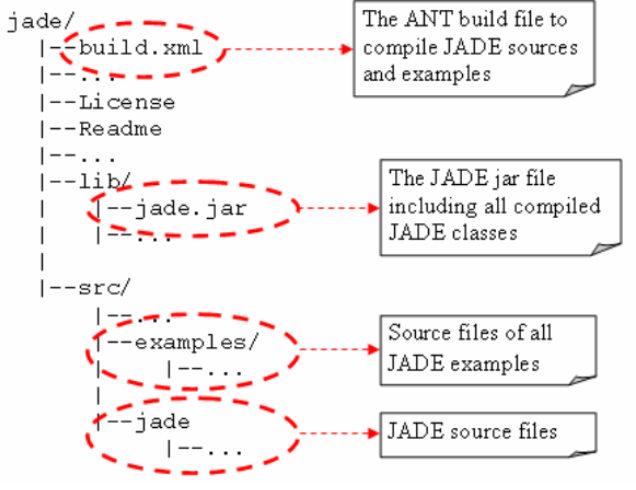
\includegraphics{images/jade.png}

\hypertarget{modo-de-ejecuciuxf3n}{%
\paragraph{Modo de ejecución}\label{modo-de-ejecuciuxf3n}}

Para lanzar la aplicación, se debe ejecutar el siguiente comando desde
el directorio Jade:

\begin{verbatim}
java -cp lib/jade.jar jade.Boot -gui
\end{verbatim}

\hypertarget{comandos-uxfatiles}{%
\paragraph{Comandos útiles}\label{comandos-uxfatiles}}

Para compilar un agente corremos el comando:

\begin{verbatim}
javac -cp lib/jade.jar -d <destino> <ruta fuente a compilar>
\end{verbatim}

Para iniciar un nuevo contenedor el comando es:

\begin{verbatim}
java -cp lib/jade.jar:classes/ jade.Boot -container
\end{verbatim}

Para iniciar un nuevo contenedor y asignarle un nombre el comando es:

\begin{verbatim}
java -cp lib/jade.jar:classes/ jade.Boot -container -container <nombre>
\end{verbatim}

Para la creación de un contenedor remoto:

\begin{verbatim}
java -cp lib/jade.jar:classes/ jade.Boot -container -host <ip_dst> -local-host <ip_src>
\end{verbatim}

    \hypertarget{c-describa-en-quuxe9-cambia-la-arquitectura-de-la-soluciuxf3n-y-cuuxe1les-son-las-ventajas-y-desventajas-comparando-esta-soluciuxf3n-con-el-estuxe1ndar-clienteservidor.}{%
\subsubsection{c) Describa en qué cambia la arquitectura de la solución
y cuáles son las ventajas y desventajas comparando esta solución con el
estándar
cliente/servidor.}\label{c-describa-en-quuxe9-cambia-la-arquitectura-de-la-soluciuxf3n-y-cuuxe1les-son-las-ventajas-y-desventajas-comparando-esta-soluciuxf3n-con-el-estuxe1ndar-clienteservidor.}}

    La arquitectura de la solución cambia en que el programador se centra en
implementar un agente, el cual se encarga de viajar hasta la máquina
remota, realizar la tarea deseada, y retornar a destino (ya no se crean
stubs como en cliente/servidor).

Mientras que en el estándar cliente/servidor, el programador se
concentra en el conjunto de métodos o procedimientos a ejecutar en la
máquina remota.

\hypertarget{ventajas}{%
\paragraph{Ventajas}\label{ventajas}}

\begin{itemize}
\tightlist
\item
  No es necesario acordar los procedimientos entre cliente y servidor.
\item
  No es necesario ejecutar una instalación del servidor.
\item
  Se evitan los constantes pedidos y respuestas propias de
  cliente/servidor, disminuyendo con esto el tráfico de la red.
\end{itemize}

\hypertarget{desventajas}{%
\paragraph{Desventajas}\label{desventajas}}

\begin{itemize}
\tightlist
\item
  Esta solución es solo compatible con la plataforma de JADE
\end{itemize}

    \hypertarget{d-identifique-las-similitudes-y-diferencias-de-distribuciuxf3nmovilidad-de-cuxf3digo-entre-rmi-y-jade.}{%
\subsubsection{d) Identifique las similitudes y diferencias de
distribución/movilidad de código entre RMI y
Jade.}\label{d-identifique-las-similitudes-y-diferencias-de-distribuciuxf3nmovilidad-de-cuxf3digo-entre-rmi-y-jade.}}

    \hypertarget{similitudes-entre-rmi-y-jad}{%
\subsubsection{Similitudes entre RMI y
Jad}\label{similitudes-entre-rmi-y-jad}}

\begin{itemize}
\tightlist
\item
  Ambas tecnologías trabajan con objetos.
\item
  Permiten la ejecución remota de código.
\item
  Ambas están implementadas en Java.
\end{itemize}

\hypertarget{diferencias-entre-rmi-y-jade}{%
\paragraph{Diferencias entre RMI y
Jade}\label{diferencias-entre-rmi-y-jade}}

\begin{itemize}
\tightlist
\item
  RMI ejecuta código que se encuentra en una máquina remota (invoca
  métodos implementados en otra máquina).
\item
  Mientras que Jade, tiene la posibilidad de migrar su código a otro
  host, ejecutarse y regresar al sitio de origen. (también permite la
  clonación de código)
\end{itemize}

    \hypertarget{programar-un-agente-muxf3vil-para-que-periuxf3dicamente-recorra-una-secuencia-de-computadoras-y-conforme-una-tabla-que-contenga}{%
\subsection{2. Programar un agente móvil para que periódicamente recorra
una secuencia de computadoras y conforme una tabla que
contenga:}\label{programar-un-agente-muxf3vil-para-que-periuxf3dicamente-recorra-una-secuencia-de-computadoras-y-conforme-una-tabla-que-contenga}}

    \hypertarget{a-la-direcciuxf3n-ip-o-nombre-de-host-de-cada-una-de-ellas.}{%
\subsubsection{a) La Dirección IP o nombre de Host de cada una de
ellas.}\label{a-la-direcciuxf3n-ip-o-nombre-de-host-de-cada-una-de-ellas.}}

    \hypertarget{b-la-hora-de-llegada-a-cada-una.}{%
\subsubsection{b) La Hora de llegada a cada
una.}\label{b-la-hora-de-llegada-a-cada-una.}}

    \hypertarget{c-la-carga-de-procesamiento-de-cada-una-de-ellas.}{%
\subsubsection{c) La carga de procesamiento de cada una de
ellas.}\label{c-la-carga-de-procesamiento-de-cada-una-de-ellas.}}

    \hypertarget{d-alguna-otra-informaciuxf3n-de-interuxe9s-que-se-le-ocurra.}{%
\subsubsection{d) Alguna otra información de interés que se le
ocurra.}\label{d-alguna-otra-informaciuxf3n-de-interuxe9s-que-se-le-ocurra.}}

    \hypertarget{al-llegar-a-cada-una-de-las-computadoras-el-agente-debe-permanecer-alluxed-al-menos-10-segundos-emitiendo-una-alerta-en-la-pantalla-local-que-indique-su-presencia.}{%
\subsubsection{Al llegar a cada una de las computadoras el agente debe
permanecer allí al menos 10 segundos, emitiendo una alerta en la
pantalla local que indique su
presencia.}\label{al-llegar-a-cada-una-de-las-computadoras-el-agente-debe-permanecer-alluxed-al-menos-10-segundos-emitiendo-una-alerta-en-la-pantalla-local-que-indique-su-presencia.}}

    \hypertarget{al-retorno-al-punto-de-origen-se-presentaruxe1-la-tabla-indicando-ademuxe1s-el-tiempo-total-ocupado-en-el-recorrido-para-recolectar-la-informaciuxf3n.}{%
\subsubsection{Al retorno al punto de origen, se presentará la tabla,
indicando además el tiempo total ocupado en el recorrido para recolectar
la
información.}\label{al-retorno-al-punto-de-origen-se-presentaruxe1-la-tabla-indicando-ademuxe1s-el-tiempo-total-ocupado-en-el-recorrido-para-recolectar-la-informaciuxf3n.}}

    \hypertarget{implementacion}{%
\paragraph{Implementacion}\label{implementacion}}

Se implementó un agente que contiene, en su método ``action()'', como
estructura principal un switch con tres opciones. Cada una de ellas es
ejecutada acorde al número de una variable estática numérica y global
que indica el ``estado'' (**\_state**) en el que se encuentra el agente.
En nuestro caso, los estados son:

\begin{itemize}
\item
  \textbf{Opción 0:} El agente está en el contenedor en que se lo
  inició. En este punto se obtiene la lista de contenedores y se prepara
  el contexto para la migración.
\item
  \textbf{Opción 1:} El agente está en alguno de los contenedores que
  deben ser escaneados para obtener información del host. Una vez
  escaneado esto, se mueve al siguiente contenedor.
\item
  \textbf{Opción 2:} El agente volvió al contenedor inicial, esto quiere
  decir que ya circulo por todos los contenedores, entonces debe
  imprimir en la salida estándar la información recolectada y terminar.
\end{itemize}

Para el guardado de la información se implementó un arreglo de la clase
``Informacion'', la cual contiene toda la especificacion de lo requerido
en cada lectura de cada contenedor. Entonces, el agente en cada
contenedor que visita instancia un objeto ``Informacion'' que contiene
toda la información escaneada y la agrega a dicho arreglo.

Luego, en el \_State=2, donde el agente ya esta nuevamente en destino y
debio haber escaneado todos los contenedores, recorre su arreglo
imprimiendo la informacion de cada objeto de tipo ``Informacion''
perteneciente a cada contenedor escaneado.

En nuestro caso, la informacion escaneada es:

\begin{itemize}
\tightlist
\item
  Host Name
\item
  IP Host
\item
  SO
\item
  Consumo de CPU
\item
  Horario de llegada al Host Destino
\item
  Horario de partida del Host
\end{itemize}

Ejemplo de Escaneo de Contenedores
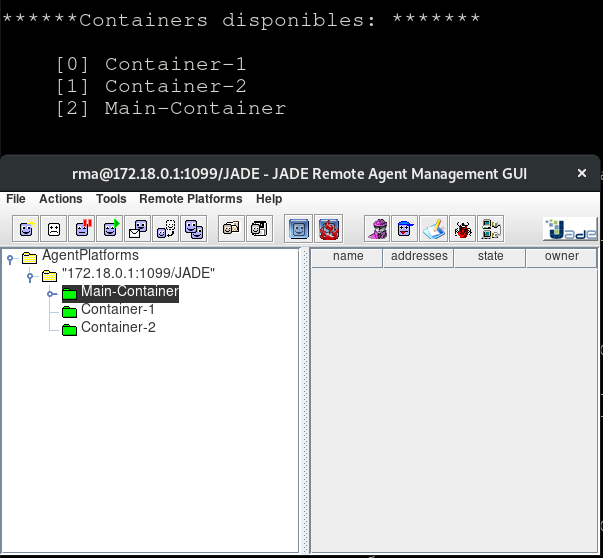
\includegraphics{images/ListadoCircular-1.png}

Ejemplo de Imprecion de un Host 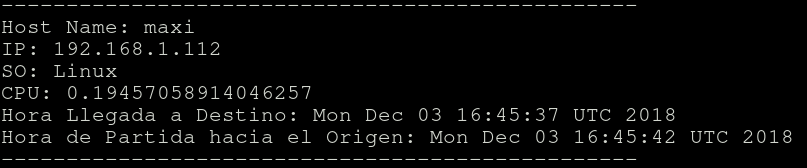
\includegraphics{images/Escaneo.png}

    \hypertarget{realizar-y-documentar-los-siguientes-experimentos}{%
\subsection{3. Realizar y documentar los siguientes
experimentos:}\label{realizar-y-documentar-los-siguientes-experimentos}}

    \hypertarget{transferir-un-archivo-de-gran-tamauxf1o-gbs-completo-las-siguientes-condiciones}{%
\subsubsection{Transferir un archivo de gran tamaño (GBs) completo las
siguientes
condiciones:}\label{transferir-un-archivo-de-gran-tamauxf1o-gbs-completo-las-siguientes-condiciones}}

    \hypertarget{a-en-la-versiuxf3n-con-java-sockets-del-tp1.}{%
\subsubsection{a) En la versión con Java Sockets del
TP1.}\label{a-en-la-versiuxf3n-con-java-sockets-del-tp1.}}

    \hypertarget{b-en-la-versiuxf3n-java-rmi-del-tp2.}{%
\subsubsection{b) En la versión Java RMI del
TP2.}\label{b-en-la-versiuxf3n-java-rmi-del-tp2.}}

    \hypertarget{c-en-la-versiuxf3n-con-agentes-muxf3viles-del-punto-1}{%
\subsubsection{c) En la versión con Agentes Móviles del punto
1}\label{c-en-la-versiuxf3n-con-agentes-muxf3viles-del-punto-1}}

    \hypertarget{utilizar-las-primitivas-de-lectura-o-escritura-con-un-tamauxf1o-de-buffer-igual-y-cronometrar-que-el-mismo-cliente-muestre-cuanto-demoruxf3-en-los-tres-casos-sacando-las-conclusiones-de-cada-caso-respecto-a-la-performance-de-cada-soluciuxf3n.-documentar-lo-realizado.}{%
\subsubsection{Utilizar las primitivas de lectura o escritura con un
tamaño de buffer igual y cronometrar (que el mismo cliente muestre
cuanto demoró), en los tres casos, sacando las conclusiones de cada caso
respecto a la performance de cada solución. Documentar lo
realizado.}\label{utilizar-las-primitivas-de-lectura-o-escritura-con-un-tamauxf1o-de-buffer-igual-y-cronometrar-que-el-mismo-cliente-muestre-cuanto-demoruxf3-en-los-tres-casos-sacando-las-conclusiones-de-cada-caso-respecto-a-la-performance-de-cada-soluciuxf3n.-documentar-lo-realizado.}}

    \hypertarget{comunicaciuxf3n-indirecta-mqtt-e-iot}{%
\section{Comunicación Indirecta: MQTT e
IoT}\label{comunicaciuxf3n-indirecta-mqtt-e-iot}}

    \hypertarget{realizar-el-siguiente-desarrollo}{%
\subsection{4. Realizar el siguiente
desarrollo}\label{realizar-el-siguiente-desarrollo}}

    \hypertarget{a.-tomar-dos-kits-de-desarrollo-galileo-o-arduino-e-instrumentar-un-protocolo-de-aplicaciuxf3n-en-modo-publicadorsuscriptor-sobre-mqtt-sobre-la-base-de-tuxf3picos-y-valores.-habruxe1-una-placa-con-sensores-y-actuadores-y-se-simularuxe1-una-aplicaciuxf3n-de-comandomonitor-mediante-mqtt-spy-java.}{%
\subsubsection{a. Tomar dos kits de desarrollo (Galileo o Arduino) e
instrumentar un protocolo de aplicación en modo Publicador/Suscriptor
sobre MQTT, sobre la base de Tópicos y valores. Habrá una placa con
sensores y actuadores y se simulará una aplicación de comando/monitor
mediante MQTT-Spy
(java).}\label{a.-tomar-dos-kits-de-desarrollo-galileo-o-arduino-e-instrumentar-un-protocolo-de-aplicaciuxf3n-en-modo-publicadorsuscriptor-sobre-mqtt-sobre-la-base-de-tuxf3picos-y-valores.-habruxe1-una-placa-con-sensores-y-actuadores-y-se-simularuxe1-una-aplicaciuxf3n-de-comandomonitor-mediante-mqtt-spy-java.}}

\hypertarget{en-la-placa-publicadora-instrumentar-una-mediciuxf3n-de-temperatura-dos-botones-por-touch-y-pulsado-como-sensores-y-dos-leds-rojo-azul-como-actuadores.-la-temperatura-se-publicaruxe1-cada-10-segundos.-el-cambio-de-estado-de-los-botones-se-publicaruxe1-cuando-ocurra-y-en-modo-eventual-con-estampa-temporal.}{%
\subsubsection{En la placa publicadora instrumentar: Una medición de
temperatura, dos botones (por touch y pulsado), como sensores y dos Leds
(Rojo azul) como actuadores. La temperatura se publicará cada 10
segundos. El cambio de estado de los botones se publicará cuando ocurra
y en modo eventual con estampa
temporal.}\label{en-la-placa-publicadora-instrumentar-una-mediciuxf3n-de-temperatura-dos-botones-por-touch-y-pulsado-como-sensores-y-dos-leds-rojo-azul-como-actuadores.-la-temperatura-se-publicaruxe1-cada-10-segundos.-el-cambio-de-estado-de-los-botones-se-publicaruxe1-cuando-ocurra-y-en-modo-eventual-con-estampa-temporal.}}

    \hypertarget{introducciuxf3n}{%
\paragraph{Introducción\\}\label{introducciuxf3n}}

La simulación de este apartado del trabajo se utilizarán las siguientes
tecnologías:

\begin{itemize}
\item
  \href{https://nodered.org/}{Node-Red}: para la simulación de la placa
  arduino y el despliegue de un panel de control
\item
  \href{https://mosquitto.org/}{Eclipse Mosquitto}: para el despliegue
  del broker
\item
  \href{https://www.docker.com/}{Docker}: para la puesta en marcha de 3
  contenedores:

  \begin{itemize}
  \item
    El broker Mosquitto que tendrá la ip \textbf{172.16.240.10}
  \item
    El nodo de Node-Red para la simulación de la placa que tendrá la ip
    \textbf{172.16.240.20}
  \item
    El node de Node-Red para el panel de control que tendrá la ip
    \textbf{172.16.240.30}
  \end{itemize}
\end{itemize}

Este ecosistema se encuentra especificado en el archivo
\textbf{\emph{docker-compose.yml}}

Para reproducir el proyecto son necesarios los siguientes pasos

\begin{enumerate}
\def\labelenumi{\arabic{enumi})}
\tightlist
\item
  \textbf{Lanzar los contenedores}
\end{enumerate}

Ejecutar el comando \texttt{docker-compose\ up\ -\/-build} en el
directorio raíz del mismo.

Luego:

\begin{itemize}
\item
  El nodo de simulación de la placa estará disponible en
  http://localhost:1880
\item
  El nodo de planel de control estará disponible en
  http://localhost:1881
\end{itemize}

\begin{enumerate}
\def\labelenumi{\arabic{enumi})}
\setcounter{enumi}{1}
\tightlist
\item
  \textbf{Importar los nodos}
\end{enumerate}

Los nodos están especificados en los archivos

\begin{itemize}
\item
  \textbf{\emph{flows/publisher/flow.json}} (simulacion arduino, puerto
  1880)
\item
  \textbf{\emph{flows/subscriber/flow.json}} (panel de control, puerto
  1881)
\end{itemize}

Los nodos se importan con \texttt{Ctrl+i} y pegando el contenido del
archivo json correspondiente en el modal. Luego presionar
\textbf{\emph{Done}} y luego \textbf{\emph{Deploy}}. Finalmente las
interfaces web estarán disponibles en las rutas:

\begin{itemize}
\item
  http://localhost:1880/ui/ (simulación arduino)
\item
  http://localhost:1881/ui/ (simulacion panel de control)
\end{itemize}

    \hypertarget{diseuxf1o}{%
\paragraph{Diseño\\}\label{diseuxf1o}}

Según los requerimientos de la consigna la placa Arduino podría tener el
siguiente esquema de conexiones:

\begin{itemize}
\item
  Un módulo ESP8266 para la conexión a la red
\item
  Un potenciómetro para simular la toma de temperatura
\item
  Dos pulsadores para la simulación de los sensores
\item
  Dos led para la simulación de los actuadores
\end{itemize}

tal como se ve en la siguiente imagen

    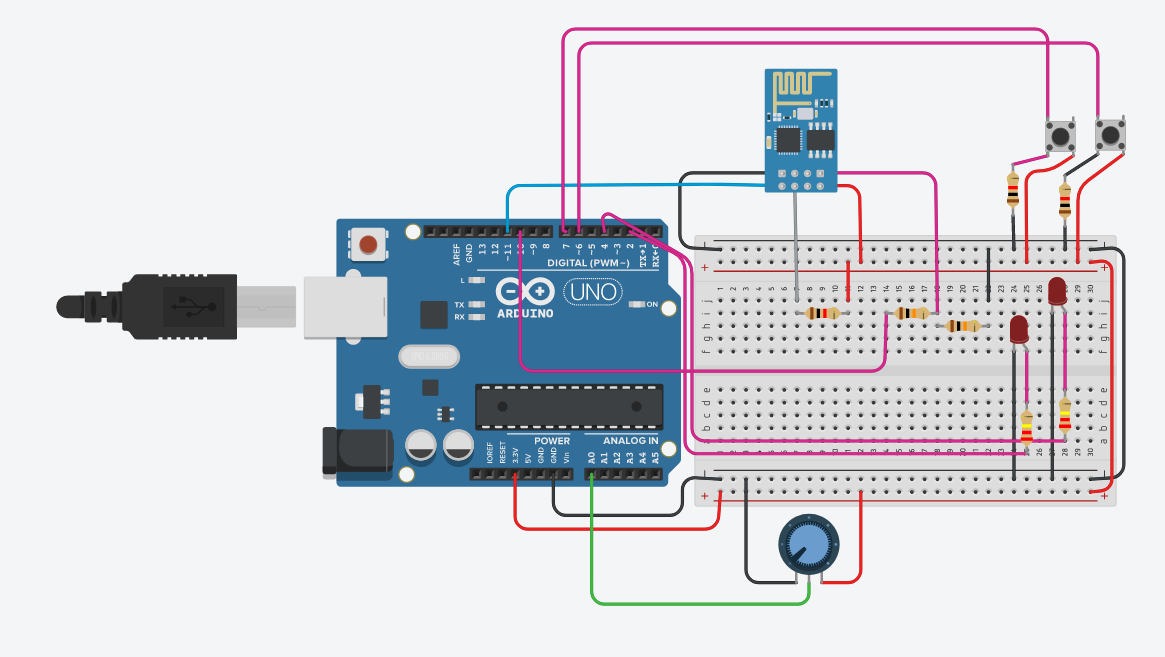
\includegraphics{images/placa.png}

    La correspondencia de este diseño arduino con la UI-web se puede ver en
la siguiente imagen

    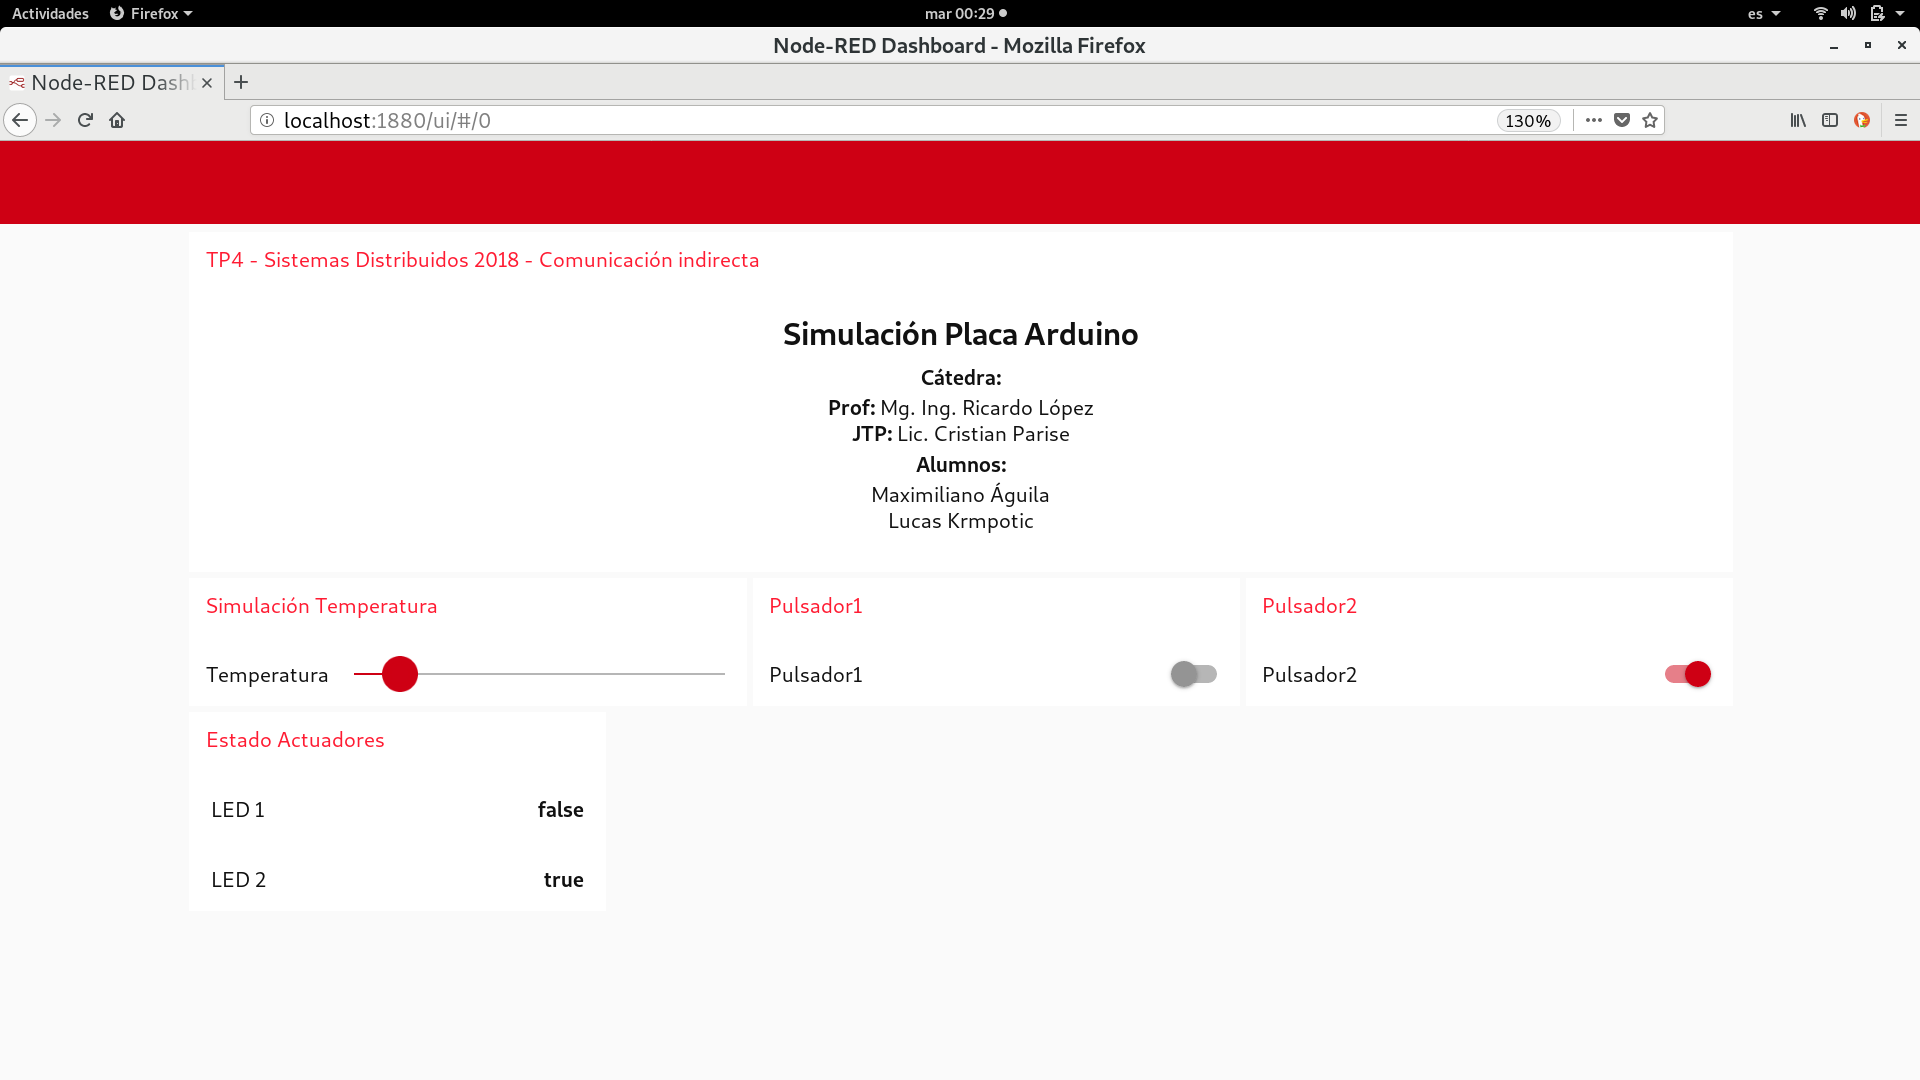
\includegraphics{images/simulacion-placa.png}

    Por su parte el panel de control cuenta con:

\begin{itemize}
\item
  Una aguja para mostrar el estado de la temperatura
\item
  Dos cajas de texto para mostrar el estado de los sensores
\item
  Dos botones para estimular los actuadores
\end{itemize}

Tal como se puede ver en la siguiente imagen:

    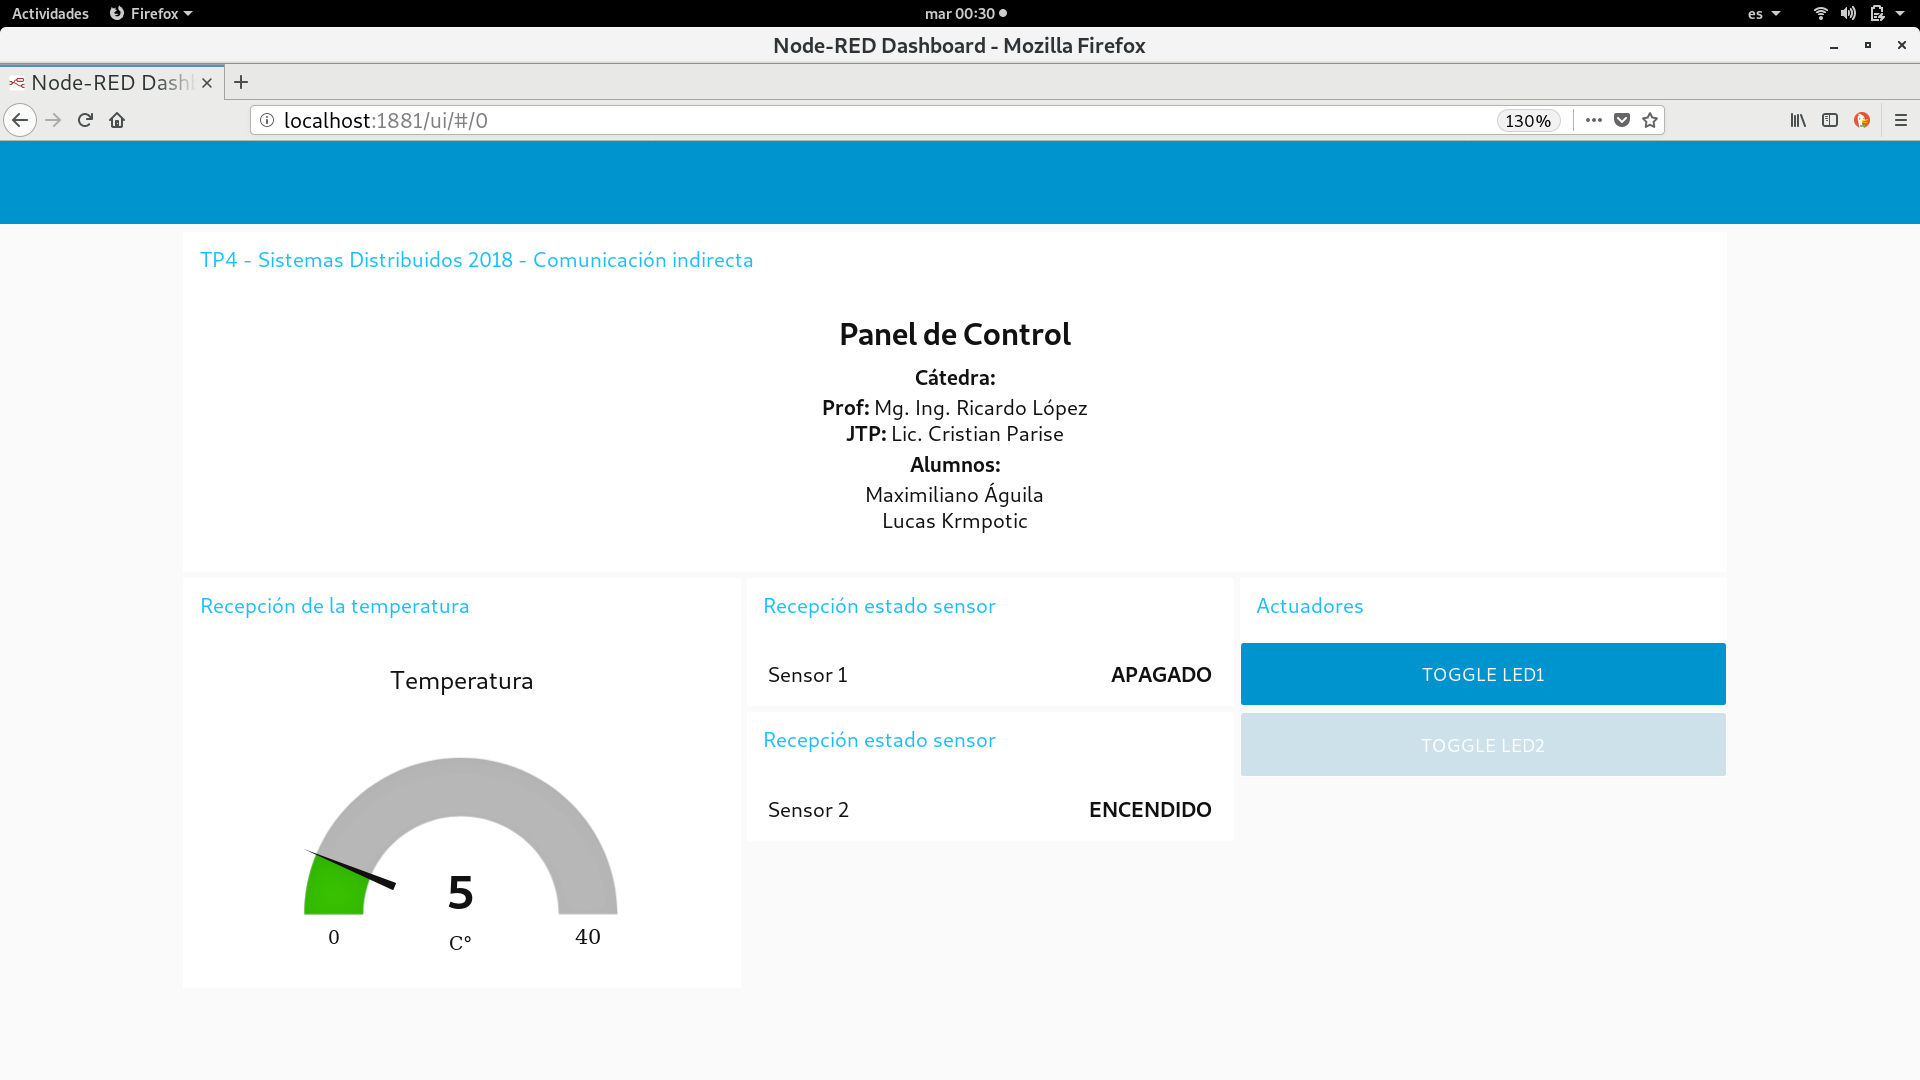
\includegraphics{images/panel-control.png}

    \hypertarget{esquema-de-tuxf3picos-y-programaciuxf3n-de-los-nodos}{%
\paragraph{Esquema de tópicos y programación de los
nodos\\}\label{esquema-de-tuxf3picos-y-programaciuxf3n-de-los-nodos}}

En sistemas grandes puede resultar conveniente la utilización de un
protocolo de aplicación (MARA por ejemplo) para publicar un conjunto
amplio de variables sobre un conjunto limitado de tópicos, lo cierto es
que en nuestro caso el problema puede resolverse con 5 tópicos que dimos
en llamar:

\begin{itemize}
\item
  \textbf{temperatura} - con arduino publicador y panel de control
  suscriptor
\item
  \textbf{pulsador1} - con arduino publicador y panel de control
  suscriptor
\item
  \textbf{pulsador2} - con arduino publicador y panel de control
  suscriptor
\item
  \textbf{Led1} - con panel de control publicador y arduino suscriptor
\item
  \textbf{Led2} - con panel de control publicador y arduino suscriptor
\end{itemize}

aprovechando las bondades de Node-Red y evitando trabajo adicional de
parseo de strings

    \hypertarget{aplicaciuxf3n-de-simulaciuxf3n-de-la-placa-arduino}{%
\subparagraph{Aplicación de simulación de la placa
Arduino}\label{aplicaciuxf3n-de-simulaciuxf3n-de-la-placa-arduino}}

En la imagen a continuación se presenta el flow correspondiente a la
aplicación que simula la placa arduino, en ella se distinguen:

\begin{itemize}
\item
  \textbf{Nodos violetas:} son nodos MQTT de entrada (suscripción) o de
  salida (publicación).
\item
  \textbf{Nodos celestes:} son nodos que definen componentes gráficos
  (html + javascript).
\item
  \textbf{Nodos azules:} son nodos de inicio que sirven para inicializar
  variables javascript con algún valor de interés
\item
  \textbf{Nodos función:} son nodos en los que se definen funciones js
  para manipular los mensajes entre los nodos.
\end{itemize}

    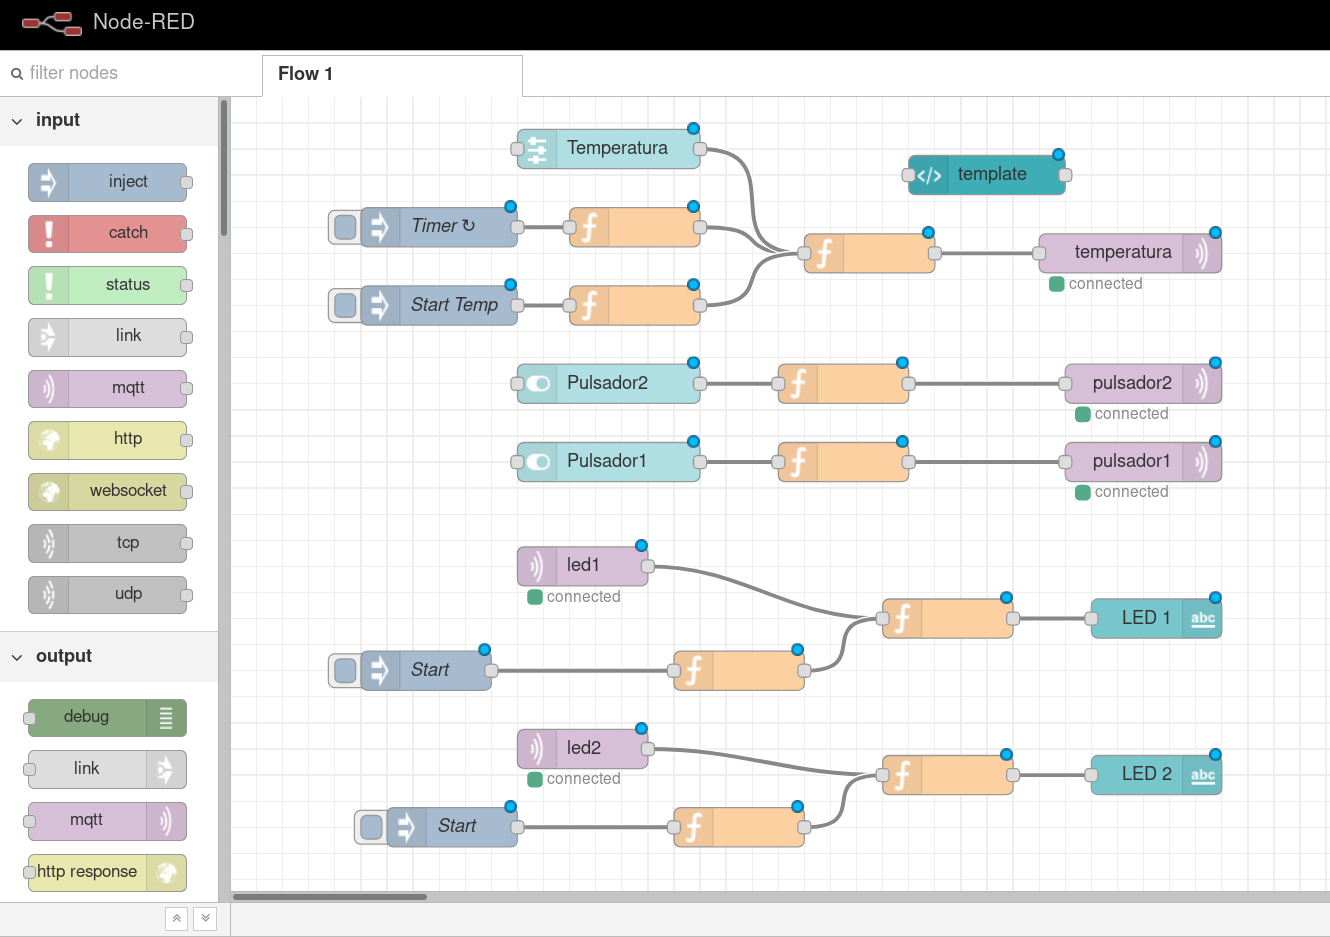
\includegraphics{images/node-red-sim-ardu.png}

    Las conexiones entre los nodos representan flujos de eventos javascript
en los que los nodos observadores reciben por parametro un objeto
llamado \textbf{\emph{msg}} que tiene un atributo llamado
\textbf{\emph{payload}} que transporta datos.

Entonces, por ejemplo, la simulación de los pulsadores hace uso del
evento propio del componente nodo \textbf{\emph{switch}} que envía
\emph{true} o \emph{false} según corresponda. El evento de cambio de
estado en el nodo switch es escuchado por el nodo función que agrega al
\emph{payload} el timesamp (como lo requería la consigna), y éste último
emite el evento escuchado por el nodo de salida MQTT que publica el
mensaje en el servidor. El código de dicho nodo función es el siguiente:

\begin{Shaded}
\begin{Highlighting}[]
\CommentTok{// recepción del mensaje con el payload (true|false) del switch}
\KeywordTok{var}\NormalTok{ estado }\OperatorTok{=} \VariableTok{msg}\NormalTok{.}\AttributeTok{payload}\OperatorTok{;}
\CommentTok{// creación del nuevo payload}
\NormalTok{_payload }\OperatorTok{=} \OperatorTok{\{\}}
\VariableTok{_payload}\NormalTok{.}\AttributeTok{estado} \OperatorTok{=}\NormalTok{ estado}\OperatorTok{;}
\VariableTok{_payload}\NormalTok{.}\AttributeTok{time} \OperatorTok{=} \KeywordTok{new} \AttributeTok{Date}\NormalTok{().}\AttributeTok{toLocaleString}\NormalTok{(}\StringTok{'es-AR'}\OperatorTok{,} \OperatorTok{\{} \DataTypeTok{timeZone}\OperatorTok{:} \StringTok{'UTC'} \OperatorTok{\}}\NormalTok{)}\OperatorTok{;}

\ControlFlowTok{return} \OperatorTok{\{}
    \DataTypeTok{payload}\OperatorTok{:}\NormalTok{_payload   }
\OperatorTok{\}}
\end{Highlighting}
\end{Shaded}

Para la publicación de la temperatura, donde el requerimiento era que se
publicase cada 10 seg, se utilizaron 2 variables con \emph{scope} más
profundo que el contexto de las funciones que intervienen en el flujo de
eventos. No estamos seguros de si se trata de variables globales o
definidas en el contexto del padre estático de las funciones del flujo,
pero para el caso es lo mismo. Persisten la ejecución de la función.

El problema es que como en Node-Red toda la programación es dirigida por
los eventos, es más natural ``descartar un mensaje'' que intentar tomar
el valor actual de una propiedad html. Una de estas variables se utilizó
para persistir el último valor de temperatura generado por el último
evento del componente \emph{slider}. La otra como flag para saber si se
cayó el timer que indica que es momento de publicar la temperatura. De
este modo cuando el splider que simula la toma de temperatura es
estimulado, el nodo función que escucha el evento de cambio de valor
hace dos cosas:

\begin{enumerate}
\def\labelenumi{\arabic{enumi})}
\item
  Guarda ese valor nuevo en la variable global \emph{temperatura}
\item
  Consulta el estado de la variable global \emph{state}, si es true
  publica ese valor y setea el flag en false, si es false no lo publica.
\end{enumerate}

Cuando el evento se produce por la caida del timer, simplemente se
publica el valor actual de la variable global temperatura y se setea el
flag en false.

El fragmento de código de la función que escucha los dos eventos es el
siguiente:

\begin{Shaded}
\begin{Highlighting}[]
\CommentTok{// si el payload es de tipo number es evento del sensor de temperatura}
\ControlFlowTok{if}\NormalTok{(}\KeywordTok{typeof} \VariableTok{msg}\NormalTok{.}\AttributeTok{payload} \OperatorTok{===} \StringTok{'number'}\NormalTok{) }\OperatorTok{\{}
    
    \CommentTok{// guarda la temperatura en la variable global}
    \VariableTok{context}\NormalTok{.}\VariableTok{global}\NormalTok{.}\AttributeTok{temperatura} \OperatorTok{=} \VariableTok{msg}\NormalTok{.}\AttributeTok{payload}\OperatorTok{;}
    
    \CommentTok{// si el flag es true la publica y setea el flag en false}
    \ControlFlowTok{if}\NormalTok{ (}\VariableTok{context}\NormalTok{.}\VariableTok{global}\NormalTok{.}\AttributeTok{state} \OperatorTok{===} \KeywordTok{true}\NormalTok{)}\OperatorTok{\{}
        \VariableTok{context}\NormalTok{.}\VariableTok{global}\NormalTok{.}\AttributeTok{state} \OperatorTok{=} \KeywordTok{false}\OperatorTok{;}
        \ControlFlowTok{return} \OperatorTok{\{}
            \DataTypeTok{payload}\OperatorTok{:} \VariableTok{context}\NormalTok{.}\VariableTok{global}\NormalTok{.}\AttributeTok{temperatura}
        \OperatorTok{\}}    
    \OperatorTok{\}}
\OperatorTok{\}}
\CommentTok{// si el payload es true es evento del timer}
\ControlFlowTok{if}\NormalTok{ (}\VariableTok{msg}\NormalTok{.}\AttributeTok{payload} \OperatorTok{===} \KeywordTok{true}\NormalTok{)}\OperatorTok{\{}
    
    \CommentTok{// setea el flag en false }
    \VariableTok{context}\NormalTok{.}\VariableTok{global}\NormalTok{.}\AttributeTok{state} \OperatorTok{=} \KeywordTok{false}\OperatorTok{;}
    
    \CommentTok{// publica la temperatura actual}
    \ControlFlowTok{return} \OperatorTok{\{}
        \DataTypeTok{payload}\OperatorTok{:} \VariableTok{context}\NormalTok{.}\VariableTok{global}\NormalTok{.}\AttributeTok{temperatura}
    \OperatorTok{\}}     
\OperatorTok{\}}
\end{Highlighting}
\end{Shaded}

    \hypertarget{aplicaciuxf3n-panel-de-control}{%
\subparagraph{Aplicación Panel de
Control}\label{aplicaciuxf3n-panel-de-control}}

Esta plicación es súmamente simple dado que no es necesario esfuerzo
adicional de formateo de mensajes.

Las únicas funciones javascript utilizadas tienen por objetivo escuchar
la recepción de mensajes en los tópicos correspondientes a los sonsores
digitales y tomar del mensaje el valor del sensor o el timestamp para
pasárselo al elemento gráfico pertinente (nodo caja de texto y nodo
notificación respectivamente).

    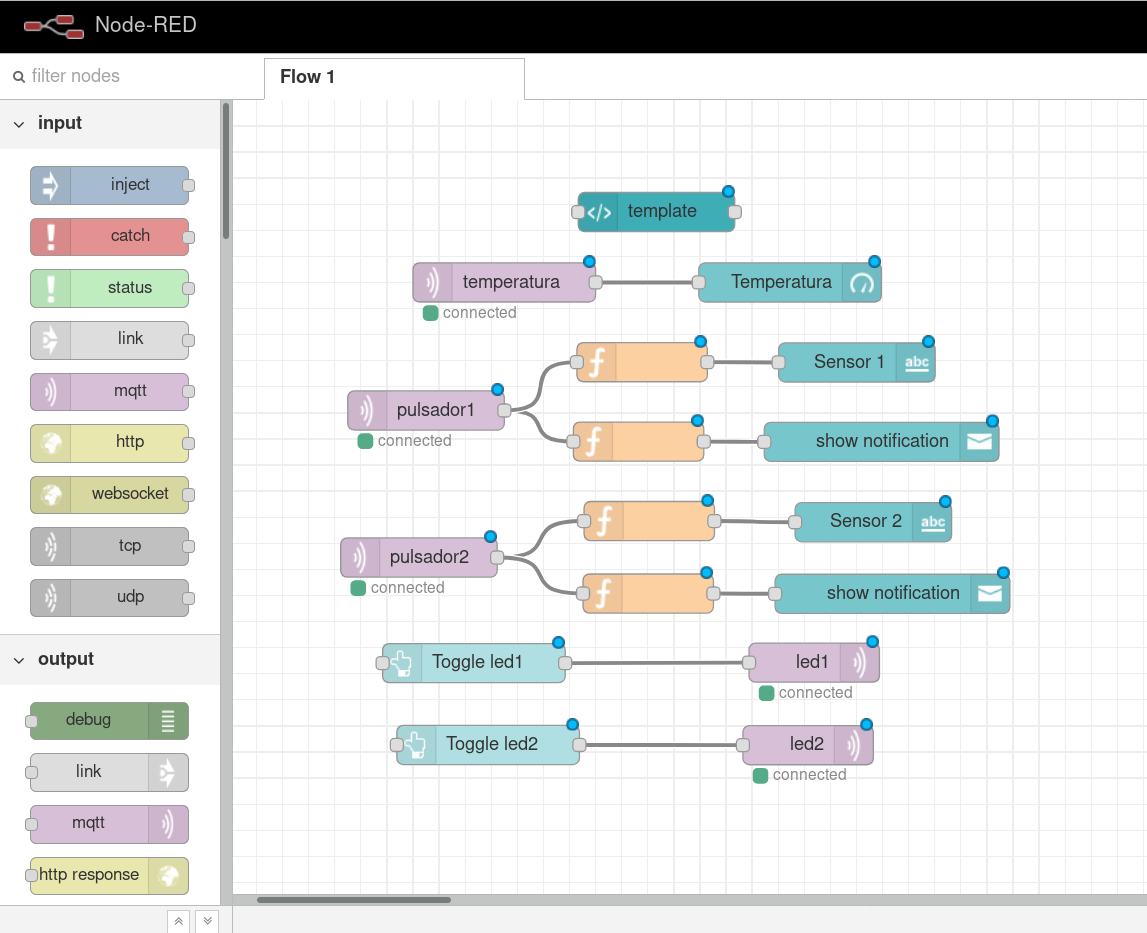
\includegraphics{images/node-red-panel-control.png}

    \hypertarget{b.-probando-con-el-servidor-mosquitto-en-localhost-analizar-mediante-wireshark-en-modo-comando-por-consola-o-utilizando-el-mqtt-spy-en-java---como-es-el-comportamiento-de-los-mensajes-variando-las-distintas-qos-0-1-y-2.-informe-lo-observado.}{%
\subsubsection{b. Probando con el servidor Mosquitto en localhost
analizar mediante wireshark --en modo comando por consola o utilizando
el MQTT-Spy en Java -, como es el comportamiento de los mensajes
variando las distintas QOS (0, 1 y 2). Informe lo
observado.}\label{b.-probando-con-el-servidor-mosquitto-en-localhost-analizar-mediante-wireshark-en-modo-comando-por-consola-o-utilizando-el-mqtt-spy-en-java---como-es-el-comportamiento-de-los-mensajes-variando-las-distintas-qos-0-1-y-2.-informe-lo-observado.}}

    \hypertarget{introducciuxf3n}{%
\paragraph{Introducción\\}\label{introducciuxf3n}}

Las calidades de servicio en MQTT determinan el modo en que se
confirmarán, o no, las recepciones de mensajes de tipo
\textbf{\emph{``Publish''}}:

\begin{itemize}
\item
  \textbf{QoS 0:} no hay confirmación
\item
  \textbf{QoS 1:} confirmación simple, receptor envía mensaje tipo
  \textbf{\emph{``Publish Ack''}}
\item
  \textbf{QoS 2:} confirmación en 2 pasos:

  \begin{itemize}
  \item
    receptor envía \textbf{\emph{``Publish Received''}}
  \item
    emisor envía \textbf{\emph{``Publish Release''}}
  \item
    receptor cierra la confirmación enviando \textbf{\emph{``Publish
    Complete''}}
  \end{itemize}
\end{itemize}

Los términos \emph{emisor} y \emph{receptor} son adecuados dado que este
comportemiento no varía por tratarse de clientes o servidores. En el
caso de un cliente publicador, la QoS se establece directamente en el
mensaje \textbf{\emph{``Publish''}}, mientras que los clientes
suscriptores requieren una determinada calidad de servicio al momento de
suscribirse a un tópico (en el campo \textbf{\emph{``Requested QoS''}}
del payload del mensaje \textbf{\emph{``Subscribe''}}).

Para probar el concepto, se usará el escenario del ejercicio anterior,
publicando mensajes al topico \emph{``pulsador1''}. El publicador
enviará siempre mensajes con QoS = 2, mientras que se variarán las
calidades de servicio en los mensajes intercambiados entre el broker y
el suscriptor.

Por una cuestión de visualización se utilizará la librería
\href{https://scapy.net/}{Scapy} de python para sniffear la red, filtrar
paquetes y disectarlos. No obstante los resultados se escribiran en
archivos \emph{pcap} que podrán ser leídos en Wireshark o herramientas
similares.

    \hypertarget{clase-sniffer-para-filtrado-y-generaciuxf3n-del-pcap}{%
\paragraph{Clase sniffer para filtrado y generación del
pcap}\label{clase-sniffer-para-filtrado-y-generaciuxf3n-del-pcap}}

    \begin{Verbatim}[commandchars=\\\{\}]
{\color{incolor}In [{\color{incolor}1}]:} \PY{k+kn}{from} \PY{n+nn}{scapy}\PY{n+nn}{.}\PY{n+nn}{all} \PY{k}{import} \PY{o}{*}
        \PY{k+kn}{from} \PY{n+nn}{scapy}\PY{n+nn}{.}\PY{n+nn}{contrib} \PY{k}{import} \PY{n}{mqtt}
        
        \PY{c+c1}{\PYZsh{} filtro paquetes tcp con origen o destino en el broker en el puerto 1883, }
        \PY{n}{FILTER}\PY{o}{=}\PY{l+s+s2}{\PYZdq{}}\PY{l+s+s2}{(dst 172.16.240.10 or scr 172.16.240.10) and tcp and dport mqtt}\PY{l+s+s2}{\PYZdq{}}
        
        \PY{k}{class} \PY{n+nc}{MQTTSniffer}\PY{p}{(}\PY{p}{)}\PY{p}{:}
            
            \PY{k}{def} \PY{n+nf}{\PYZus{}\PYZus{}init\PYZus{}\PYZus{}}\PY{p}{(}\PY{n+nb+bp}{self}\PY{p}{)}\PY{p}{:}
                \PY{n+nb+bp}{self}\PY{o}{.}\PY{n}{packets} \PY{o}{=} \PY{p}{[}\PY{p}{]}
            
            \PY{k}{def} \PY{n+nf}{pkt\PYZus{}save}\PY{p}{(}\PY{n+nb+bp}{self}\PY{p}{,} \PY{n}{pkt}\PY{p}{)}\PY{p}{:}
                \PY{l+s+sd}{\PYZdq{}\PYZdq{}\PYZdq{} guarda el paquete en la lista controlando que sea MQTT \PYZdq{}\PYZdq{}\PYZdq{}}
                \PY{k}{if} \PY{n}{pkt}\PY{o}{.}\PY{n}{haslayer}\PY{p}{(}\PY{n}{mqtt}\PY{o}{.}\PY{n}{MQTT}\PY{p}{)}\PY{p}{:}
                    \PY{n+nb+bp}{self}\PY{o}{.}\PY{n}{packets}\PY{o}{.}\PY{n}{append}\PY{p}{(}\PY{n}{pkt}\PY{p}{)}
                    
            \PY{k}{def} \PY{n+nf}{to\PYZus{}pcap}\PY{p}{(}\PY{n+nb+bp}{self}\PY{p}{,} \PY{n}{file\PYZus{}name}\PY{p}{)}\PY{p}{:}
                \PY{l+s+sd}{\PYZdq{}\PYZdq{}\PYZdq{} genera un archivo pcap con la lista de paquetes \PYZdq{}\PYZdq{}\PYZdq{}}
                \PY{n}{wrpcap}\PY{p}{(}\PY{n}{file\PYZus{}name}\PY{p}{,} \PY{n+nb+bp}{self}\PY{o}{.}\PY{n}{packets}\PY{p}{)}
\end{Verbatim}


    \hypertarget{prueba-1-qos-2-en-publicador-qos-0-en-suscriptor}{%
\paragraph{Prueba 1: QoS 2 en publicador, QoS 0 en
suscriptor}\label{prueba-1-qos-2-en-publicador-qos-0-en-suscriptor}}

Escenario teórico esperado:\\:

    \begin{center}
    \adjustimage{max size={0.9\linewidth}{0.9\paperheight}}{images/qos0.png}
    \end{center}

    Ejecucion de la prueba

    \begin{Verbatim}[commandchars=\\\{\}]
{\color{incolor}In [{\color{incolor}140}]:} \PY{c+c1}{\PYZsh{} instanciamos nuestro sniffer}
          \PY{n}{sniffer} \PY{o}{=} \PY{n}{MQTTSniffer}\PY{p}{(}\PY{p}{)}
          
          \PY{c+c1}{\PYZsh{} lo ponemos a sniffear 25 paquetes en la interfaz Docker que funciona como gateway}
          \PY{n}{sniff}\PY{p}{(}\PY{n}{iface}\PY{o}{=}\PY{l+s+s2}{\PYZdq{}}\PY{l+s+s2}{br\PYZhy{}b1e46316c5ac}\PY{l+s+s2}{\PYZdq{}}\PY{p}{,} \PY{n+nb}{filter}\PY{o}{=}\PY{n}{FILTER}\PY{p}{,} \PY{n}{prn}\PY{o}{=}\PY{n}{sniffer}\PY{o}{.}\PY{n}{pkt\PYZus{}save}\PY{p}{,} \PY{n}{count}\PY{o}{=}\PY{l+m+mi}{25}\PY{p}{)}
          
          \PY{c+c1}{\PYZsh{} escribimos el resultado en un archivo pcap}
          \PY{n}{sniffer}\PY{o}{.}\PY{n}{to\PYZus{}pcap}\PY{p}{(}\PY{l+s+s2}{\PYZdq{}}\PY{l+s+s2}{QoS\PYZhy{}0.pcap}\PY{l+s+s2}{\PYZdq{}}\PY{p}{)}
          
          \PY{c+c1}{\PYZsh{} mostramos el resultado en pantalla}
          \PY{p}{[}\PY{n}{pkt}\PY{o}{.}\PY{n}{summary}\PY{p}{(}\PY{p}{)} \PY{k}{for} \PY{n}{pkt} \PY{o+ow}{in} \PY{n}{sniffer}\PY{o}{.}\PY{n}{packets}\PY{p}{]}
\end{Verbatim}


\begin{Verbatim}[commandchars=\\\{\}]
{\color{outcolor}Out[{\color{outcolor}140}]:} ['Ether / IP / TCP 172.16.240.20:59718 > 172.16.240.10:mqtt PA / MQTT / MQTTPublish',
           'Ether / IP / TCP 172.16.240.10:mqtt > 172.16.240.20:59718 PA / MQTT / MQTTPubrec',
           'Ether / IP / TCP 172.16.240.20:59718 > 172.16.240.10:mqtt PA / MQTT / MQTTPubrel',
           'Ether / IP / TCP 172.16.240.10:mqtt > 172.16.240.20:59718 PA / MQTT / MQTTPubcomp',
           'Ether / IP / TCP 172.16.240.10:mqtt > 172.16.240.30:45220 PA / MQTT / MQTTPublish']
\end{Verbatim}
            
    Vemos que efectivamente el sniffer capturó 5 paquetes correspondientes a
los intercambios publicador/broker/suscriptor y que son consistentes con
el Escenario teórico esperado:\\.

Finalmente ploteamos la disección del último paquete que corresponde al
envío del mensaje desde el broker al suscriptor. En la imagen podemos
ver que el campo QoS tiene el valor \textbf{\emph{At most once
delivery}}, versión verbosa de QoS=0.

    \begin{Verbatim}[commandchars=\\\{\}]
{\color{incolor}In [{\color{incolor}4}]:} \PY{n}{cap}\PY{o}{=}\PY{n}{rdpcap}\PY{p}{(}\PY{l+s+s2}{\PYZdq{}}\PY{l+s+s2}{QoS\PYZhy{}0.pcap}\PY{l+s+s2}{\PYZdq{}}\PY{p}{)}
        \PY{n}{cap}\PY{p}{[}\PY{l+m+mi}{4}\PY{p}{]}\PY{o}{.}\PY{n}{canvas\PYZus{}dump}\PY{p}{(}\PY{p}{)}
\end{Verbatim}


    \begin{Verbatim}[commandchars=\\\{\}]
Ignoring line 5841 in mapping file 'psfonts.map': Unknown token '<DSSerif-Bold'
Ignoring line 5843 in mapping file 'psfonts.map': Unknown token '<DSSerifUni-Bold'
Ignoring line 5841 in mapping file 'psfonts.map': Unknown token '<DSSerif-Bold'
Ignoring line 5843 in mapping file 'psfonts.map': Unknown token '<DSSerifUni-Bold'

    \end{Verbatim}
\texttt{\color{outcolor}Out[{\color{outcolor}4}]:}
    
    \begin{center}
    \adjustimage{max size={0.9\linewidth}{0.9\paperheight}}{Laboratorio-4_files/Laboratorio-4_48_1.pdf}
    \end{center}
    { \hspace*{\fill} \\}
    

    \hypertarget{prueba-2-qos-2-en-publicador-qos-1-en-suscriptor}{%
\paragraph{Prueba 2: QoS 2 en publicador QoS 1 en
suscriptor}\label{prueba-2-qos-2-en-publicador-qos-1-en-suscriptor}}

Escenario teórico esperado:\\

    \begin{center}
    \adjustimage{max size={0.9\linewidth}{0.9\paperheight}}{images/qos1.png}
    \end{center}


    Ejecución de la prueba

    \begin{Verbatim}[commandchars=\\\{\}]
{\color{incolor}In [{\color{incolor}3}]:} \PY{n}{sniffer} \PY{o}{=} \PY{n}{MQTTSniffer}\PY{p}{(}\PY{p}{)}
        \PY{n}{sniff}\PY{p}{(}\PY{n}{iface}\PY{o}{=}\PY{l+s+s2}{\PYZdq{}}\PY{l+s+s2}{br\PYZhy{}b1e46316c5ac}\PY{l+s+s2}{\PYZdq{}}\PY{p}{,} \PY{n+nb}{filter}\PY{o}{=}\PY{n}{FILTER}\PY{p}{,} \PY{n}{prn}\PY{o}{=}\PY{n}{sniffer}\PY{o}{.}\PY{n}{pkt\PYZus{}save}\PY{p}{,} \PY{n}{count}\PY{o}{=}\PY{l+m+mi}{25}\PY{p}{)}
        \PY{n}{sniffer}\PY{o}{.}\PY{n}{to\PYZus{}pcap}\PY{p}{(}\PY{l+s+s2}{\PYZdq{}}\PY{l+s+s2}{QoS\PYZhy{}1.pcap}\PY{l+s+s2}{\PYZdq{}}\PY{p}{)}
        \PY{p}{[}\PY{n}{pkt}\PY{o}{.}\PY{n}{summary}\PY{p}{(}\PY{p}{)} \PY{k}{for} \PY{n}{pkt} \PY{o+ow}{in} \PY{n}{sniffer}\PY{o}{.}\PY{n}{packets}\PY{p}{]}
\end{Verbatim}


\begin{Verbatim}[commandchars=\\\{\}]
{\color{outcolor}Out[{\color{outcolor}3}]:} ['Ether / IP / TCP 172.16.240.20:59718 > 172.16.240.10:mqtt PA / MQTT / MQTTPublish',
         'Ether / IP / TCP 172.16.240.10:mqtt > 172.16.240.20:59718 PA / MQTT / MQTTPubrec',
         'Ether / IP / TCP 172.16.240.20:59718 > 172.16.240.10:mqtt PA / MQTT / MQTTPubrel',
         'Ether / IP / TCP 172.16.240.10:mqtt > 172.16.240.20:59718 PA / MQTT / MQTTPubcomp',
         'Ether / IP / TCP 172.16.240.10:mqtt > 172.16.240.30:48994 PA / MQTT / MQTTPublish',
         'Ether / IP / TCP 172.16.240.30:48994 > 172.16.240.10:mqtt PA / MQTT / MQTTPuback']
\end{Verbatim}
            
    Nuevamente el escenario es el esperado y en la imagen del mensaje
\textbf{\emph{``Publish''}} desde el broker al suscriptor podemos
comprobar que el campo QoS tiene el valor \textbf{\emph{``At least once
delivery''}} (QoS=1).

    \begin{Verbatim}[commandchars=\\\{\}]
{\color{incolor}In [{\color{incolor}2}]:} \PY{n}{cap}\PY{o}{=}\PY{n}{rdpcap}\PY{p}{(}\PY{l+s+s2}{\PYZdq{}}\PY{l+s+s2}{QoS\PYZhy{}1.pcap}\PY{l+s+s2}{\PYZdq{}}\PY{p}{)}
        \PY{n}{cap}\PY{p}{[}\PY{l+m+mi}{4}\PY{p}{]}\PY{o}{.}\PY{n}{canvas\PYZus{}dump}\PY{p}{(}\PY{p}{)}
\end{Verbatim}


    \begin{Verbatim}[commandchars=\\\{\}]
Ignoring line 5841 in mapping file 'psfonts.map': Unknown token '<DSSerif-Bold'
Ignoring line 5843 in mapping file 'psfonts.map': Unknown token '<DSSerifUni-Bold'
Ignoring line 5841 in mapping file 'psfonts.map': Unknown token '<DSSerif-Bold'
Ignoring line 5843 in mapping file 'psfonts.map': Unknown token '<DSSerifUni-Bold'

    \end{Verbatim}
\texttt{\color{outcolor}Out[{\color{outcolor}2}]:}
    
    \begin{center}
    \adjustimage{max size={0.9\linewidth}{0.9\paperheight}}{Laboratorio-4_files/Laboratorio-4_54_1.pdf}
    \end{center}
    { \hspace*{\fill} \\}
    

    \hypertarget{prueba-3-qos-2-en-publicador-qos-2-en-suscriptor}{%
\paragraph{Prueba 3: QoS 2 en publicador, QoS 2 en
suscriptor}\label{prueba-3-qos-2-en-publicador-qos-2-en-suscriptor}}

Escenario teórico esperado:\\

    \begin{center}
    \adjustimage{max size={0.9\linewidth}{0.9\paperheight}}{images/qos2.png}
    \end{center}


    Ejecución de la prueba

    \begin{Verbatim}[commandchars=\\\{\}]
{\color{incolor}In [{\color{incolor}4}]:} \PY{n}{sniffer} \PY{o}{=} \PY{n}{MQTTSniffer}\PY{p}{(}\PY{p}{)}
        \PY{n}{sniff}\PY{p}{(}\PY{n}{iface}\PY{o}{=}\PY{l+s+s2}{\PYZdq{}}\PY{l+s+s2}{br\PYZhy{}b1e46316c5ac}\PY{l+s+s2}{\PYZdq{}}\PY{p}{,} \PY{n+nb}{filter}\PY{o}{=}\PY{n}{FILTER}\PY{p}{,} \PY{n}{prn}\PY{o}{=}\PY{n}{sniffer}\PY{o}{.}\PY{n}{pkt\PYZus{}save}\PY{p}{,} \PY{n}{count}\PY{o}{=}\PY{l+m+mi}{25}\PY{p}{)}
        \PY{n}{sniffer}\PY{o}{.}\PY{n}{to\PYZus{}pcap}\PY{p}{(}\PY{l+s+s2}{\PYZdq{}}\PY{l+s+s2}{QoS\PYZhy{}2.pcap}\PY{l+s+s2}{\PYZdq{}}\PY{p}{)}
        \PY{p}{[}\PY{n}{pkt}\PY{o}{.}\PY{n}{summary}\PY{p}{(}\PY{p}{)} \PY{k}{for} \PY{n}{pkt} \PY{o+ow}{in} \PY{n}{sniffer}\PY{o}{.}\PY{n}{packets}\PY{p}{]}
\end{Verbatim}


\begin{Verbatim}[commandchars=\\\{\}]
{\color{outcolor}Out[{\color{outcolor}4}]:} ['Ether / IP / TCP 172.16.240.20:59718 > 172.16.240.10:mqtt PA / MQTT / MQTTPublish',
         'Ether / IP / TCP 172.16.240.10:mqtt > 172.16.240.20:59718 PA / MQTT / MQTTPubrec',
         'Ether / IP / TCP 172.16.240.20:59718 > 172.16.240.10:mqtt PA / MQTT / MQTTPubrel',
         'Ether / IP / TCP 172.16.240.10:mqtt > 172.16.240.20:59718 PA / MQTT / MQTTPubcomp',
         'Ether / IP / TCP 172.16.240.10:mqtt > 172.16.240.30:49106 PA / MQTT / MQTTPublish',
         'Ether / IP / TCP 172.16.240.30:49106 > 172.16.240.10:mqtt PA / MQTT / MQTTPubrec',
         'Ether / IP / TCP 172.16.240.10:mqtt > 172.16.240.30:49106 PA / MQTT / MQTTPubrel',
         'Ether / IP / TCP 172.16.240.30:49106 > 172.16.240.10:mqtt PA / MQTT / MQTTPubcomp']
\end{Verbatim}
            
    Efectivamente 8 paquetes han sido capturados y el ploteo del mensaje
muestra que el campo QoS tiene el valor \textbf{\emph{``Exactly once
delivery''}} (QoS=2).

    \begin{Verbatim}[commandchars=\\\{\}]
{\color{incolor}In [{\color{incolor}3}]:} \PY{n}{cap}\PY{o}{=}\PY{n}{rdpcap}\PY{p}{(}\PY{l+s+s2}{\PYZdq{}}\PY{l+s+s2}{QoS\PYZhy{}2.pcap}\PY{l+s+s2}{\PYZdq{}}\PY{p}{)}
        \PY{n}{cap}\PY{p}{[}\PY{l+m+mi}{4}\PY{p}{]}\PY{o}{.}\PY{n}{canvas\PYZus{}dump}\PY{p}{(}\PY{p}{)}
\end{Verbatim}


    \begin{Verbatim}[commandchars=\\\{\}]
Ignoring line 5841 in mapping file 'psfonts.map': Unknown token '<DSSerif-Bold'
Ignoring line 5843 in mapping file 'psfonts.map': Unknown token '<DSSerifUni-Bold'
Ignoring line 5841 in mapping file 'psfonts.map': Unknown token '<DSSerif-Bold'
Ignoring line 5843 in mapping file 'psfonts.map': Unknown token '<DSSerifUni-Bold'

    \end{Verbatim}
\texttt{\color{outcolor}Out[{\color{outcolor}3}]:}
    
    \begin{center}
    \adjustimage{max size={0.9\linewidth}{0.9\paperheight}}{Laboratorio-4_files/Laboratorio-4_60_1.pdf}
    \end{center}
    { \hspace*{\fill} \\}
    

    \hypertarget{c.-investigar-sobre-android-utilizando-una-app-de-mqtt-ej-mqtt-dashboard-y-publicar-mensajes-del-protocolo-de-aplicaciuxf3n-desarrollado-en-el-apartado-a-para-controlar-y-monitorear-los-sensores-y-actuadores-de-la-placa.}{%
\subsubsection{c. Investigar sobre ANDROID utilizando una app de MQTT
(ej: Mqtt DashBoard) y publicar mensajes del protocolo de aplicación
desarrollado en el apartado a) para controlar y monitorear los sensores
y actuadores de la
placa.}\label{c.-investigar-sobre-android-utilizando-una-app-de-mqtt-ej-mqtt-dashboard-y-publicar-mensajes-del-protocolo-de-aplicaciuxf3n-desarrollado-en-el-apartado-a-para-controlar-y-monitorear-los-sensores-y-actuadores-de-la-placa.}}

    A continuación se presentan 2 capturas de pantalla que documentan el uso
de la aplicación MQTT Dashboard en el marco del escenario desarrollado
en el incisa a).

La primera imagen muestra como es posible suscribirse al tópico
temperatura y la segunda muestra la creación de 2 botones para hacer
toggle sobre los actuadores, publicando sobre los tópicos led1 y led2.

    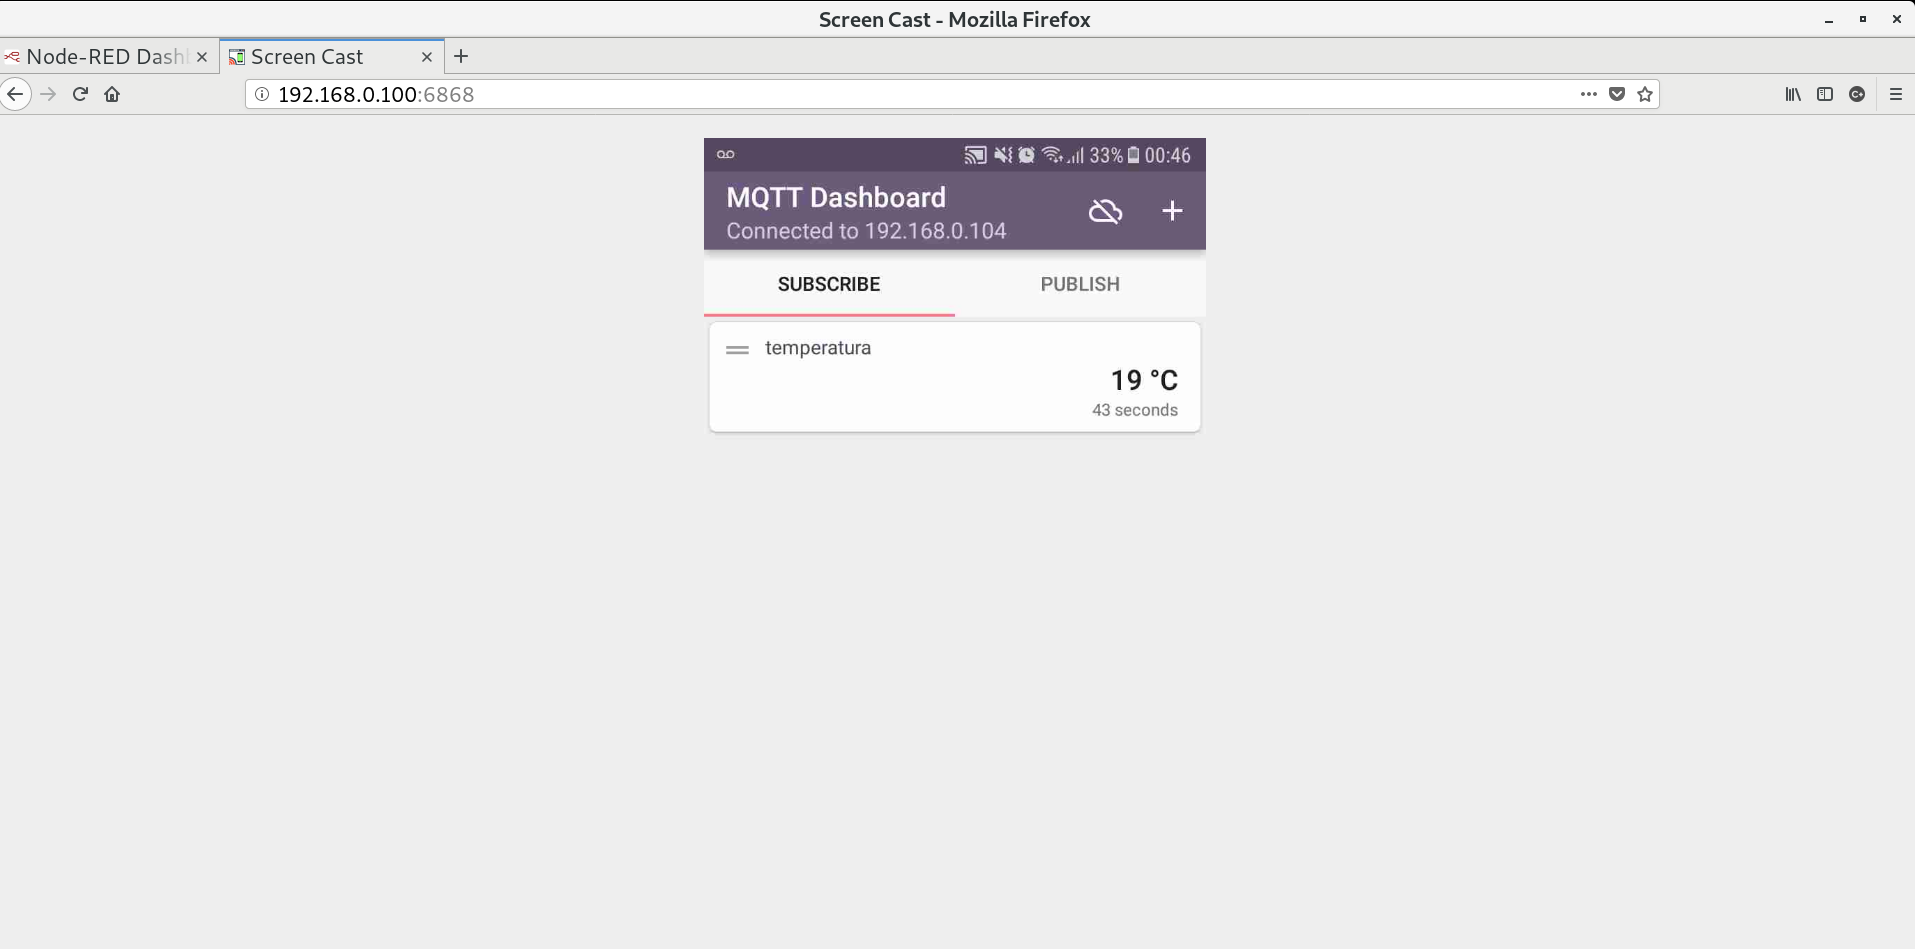
\includegraphics{images/dashboard-subs.png}

    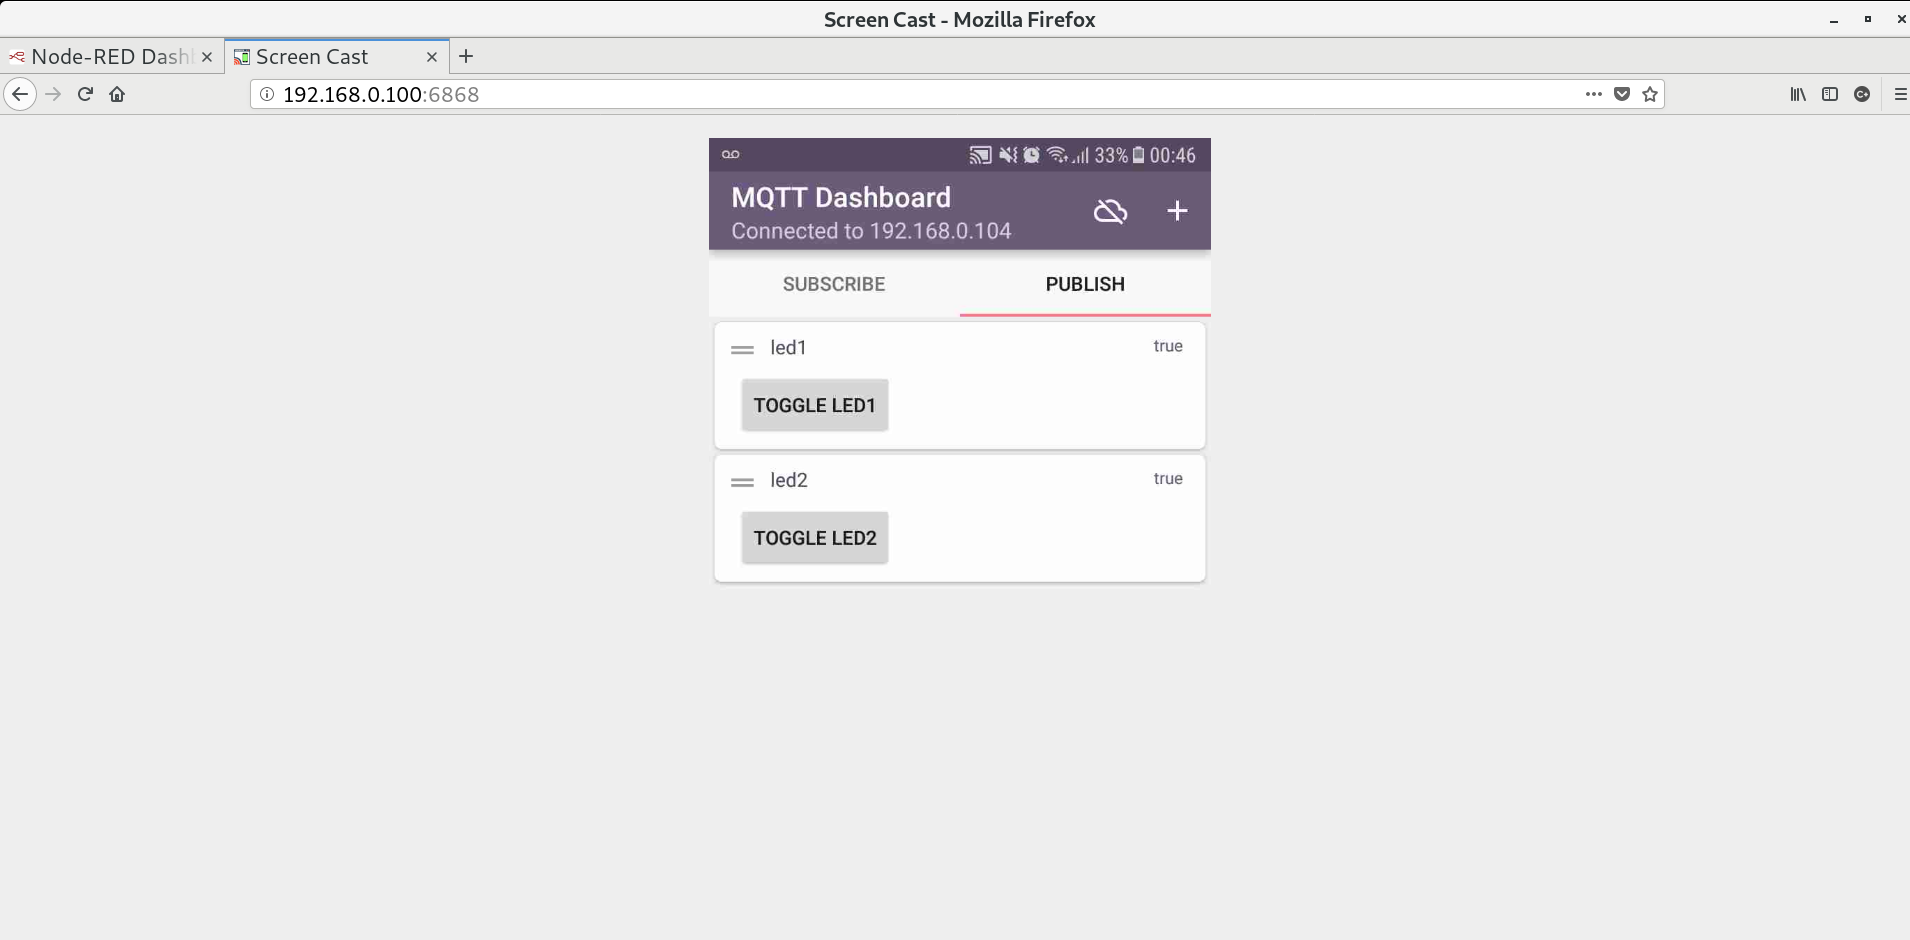
\includegraphics{images/dashboard-pub.png}

    Cabe mencionar que en el escenario planteado no se hizo huso de
autenticación para la publicación/suscripcipón en los tópicos.


    % Add a bibliography block to the postdoc
    
    
    
    \end{document}
